\clearpage

\phantomsection

\setcounter{chapter}{1}
\chapter[{KIẾN TRÚC MÔ HÌNH AnimeGANv3 (DTGAN)}]{KIẾN TRÚC MÔ HÌNH AnimeGANv3 (DTGAN)}

Chương này trình bày chi tiết kiến trúc kỹ thuật của mô hình AnimeGANv3, hay còn gọi là DTGAN (\textit{Double-Tail Generative Adversarial Network}), được đề xuất bởi Liu et al. \cite{Liu2024} vào năm 2024. Đây là chương trọng tâm kỹ thuật của luận văn, bao gồm: tổng quan kiến trúc hai nhánh, cơ chế chuẩn hóa LADE, cơ chế chú ý External Attention v3, kiến trúc Discriminator, hệ thống hàm mất mát đa thành phần, và quy trình huấn luyện theo hai giai đoạn.

Cách trình bày trong chương tuân theo nguyên tắc thống nhất: mỗi thành phần kiến trúc được mô tả theo trình tự \textbf{động lực thiết kế} $\rightarrow$ \textbf{công thức toán học} $\rightarrow$ \textbf{diễn giải ý nghĩa từng số hạng} $\rightarrow$ \textbf{nhận xét, đánh giá}. Mục tiêu là làm rõ không chỉ ``mô hình hoạt động như thế nào'' mà còn ``vì sao các tác giả lựa chọn thiết kế đó'' và ``lựa chọn đó đánh đổi những gì''.

% =====================================================
\section{Tổng quan kiến trúc DTGAN}
\label{sec:dtgan_overview}

\subsection{Động lực thiết kế: vì sao cần kiến trúc hai nhánh}
\label{subsec:why_double_tail}

Quan sát kỹ phong cách anime cho thấy hai thuộc tính thị giác có bản chất rất khác nhau cùng tồn tại trong một bức ảnh:

\begin{enumerate}
    \item \textbf{Hệ thống đường nét và cấu trúc hình khối sáng tối} -- các đường viền đậm, sắc, liên tục; sự phân tách rõ ràng giữa vùng sáng và vùng tối. Đặc trưng này mang tính \textit{tần số cao} (high-frequency), phụ thuộc vào gradient cục bộ và gần như độc lập với màu sắc.
    \item \textbf{Phân phối màu phẳng kiểu cel-shading} -- các mảng màu lớn đồng nhất, ít biến thiên kết cấu bên trong. Đặc trưng này mang tính \textit{tần số thấp} (low-frequency), phụ thuộc vào thống kê màu toàn cục và bị phá vỡ nếu mô hình cố gắng giữ lại chi tiết kết cấu.
\end{enumerate}

Hai mục tiêu này \textbf{mâu thuẫn trực tiếp} với nhau khi tối ưu trên cùng một tập tham số. Cụ thể, gọi $\theta$ là tham số của một decoder duy nhất, và $\mathcal{L}_{\text{edge}}$, $\mathcal{L}_{\text{flat}}$ lần lượt là hàm mất mát cho hai mục tiêu trên. Bài toán tối ưu hợp nhất có dạng:

\begin{equation}
\label{eq:conflict_objective}
\theta^* = \arg\min_{\theta} \Big[ \underbrace{\mathcal{L}_{\text{edge}}(\theta)}_{\text{cần gradient lớn tại biên}} + \underbrace{\mathcal{L}_{\text{flat}}(\theta)}_{\text{cần gradient nhỏ trong vùng}} \Big]
\end{equation}

Gradient của hai số hạng có xu hướng ngược chiều nhau tại các pixel nằm gần biên: $\mathcal{L}_{\text{edge}}$ khuyến khích mạng \textit{khuếch đại} chênh lệch cường độ, trong khi $\mathcal{L}_{\text{flat}}$ khuyến khích mạng \textit{triệt tiêu} chênh lệch đó. Nghiệm $\theta^*$ vì vậy là một điểm thỏa hiệp: đường nét không đủ sắc \textit{và} vùng màu không đủ phẳng.

DTGAN giải quyết mâu thuẫn này bằng cách \textbf{tách không gian tham số}: mỗi mục tiêu được giao cho một decoder riêng với bộ trọng số độc lập, trong khi phần trích xuất đặc trưng ngữ nghĩa (vốn chung cho cả hai) được chia sẻ.

\subsection{Ba thành phần của Generator}
\label{subsec:three_components}

Generator được chia thành ba thành phần \cite{Liu2024}:

\begin{itemize}
    \item \textbf{Base Encoder (Mạng mã hóa dùng chung):} Tiếp nhận ảnh gốc, trích xuất đặc trưng ngữ nghĩa phân cấp qua 3 lần downsampling (stride-2), thu nhỏ không gian ảnh thành bản đồ đặc trưng $32 \times 32$. Thiết kế dùng chung (shared weights) đảm bảo cả hai nhánh decoder khởi nguồn từ cùng một không gian đặc trưng thống nhất, đồng thời giảm đáng kể số tham số.
    \item \textbf{Support Tail (Nhánh hỗ trợ):} Sinh ảnh anime thô $\widehat{y}_s$, sau đó qua bộ lọc bảo toàn cạnh Guided Filter tạo ảnh $\widehat{y}$. Ảnh này được chuyển sang grayscale trước khi đưa vào Discriminator, buộc nhánh tập trung vào đường nét và tương phản sáng tối mà không bị phân tâm bởi màu sắc.
    \item \textbf{Main Tail (Nhánh chính):} Sinh ảnh anime hoàn chỉnh $\widehat{y}_m$ với phân phối màu sắc cel-shading mịn. Nhánh này được tối ưu dựa trên pseudo ground-truth (ảnh đã qua NL-Means + L0 Smoothing), đảm bảo vùng màu phẳng và không có lỗi đồ họa (artifacts).
\end{itemize}

\begin{figure}[H]
    \centering
    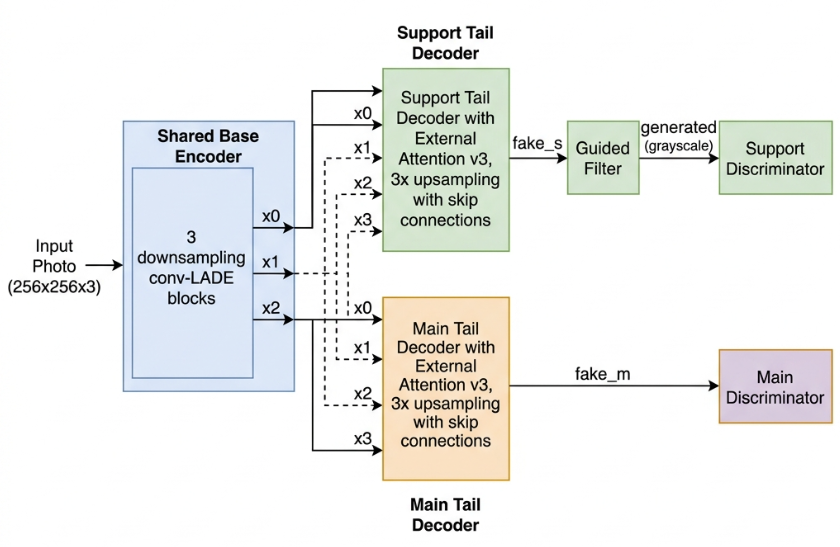
\includegraphics[width=0.95\textwidth]{figChap2/dtgan_architecture.png}
    \caption{Tổng quan kiến trúc DTGAN (AnimeGANv3)}
    \label{fig:dtgan_architecture}
\end{figure}
    \noindent\textit{Chú thích:} Ảnh đầu vào qua Shared Base Encoder để tạo các bản đồ đặc trưng $x_0, x_1, x_2, x_3$, sau đó được xử lý song song bởi Support Tail và Main Tail với skip connections kiểu U-Net. Output của Support Tail qua Guided Filter trước khi đưa vào Discriminator grayscale \cite{Liu2024}

\textbf{Điểm quan trọng cần lưu ý:} chỉ có \textbf{Main Tail} được sử dụng ở giai đoạn suy luận (inference). Support Tail cùng toàn bộ hai Discriminator là ``giàn giáo huấn luyện'' (training scaffold) -- chúng định hình gradient cho Base Encoder trong quá trình học nhưng bị loại bỏ khi xuất mô hình sang ONNX. Đây là lý do model triển khai chỉ nặng 9,1~MB dù kiến trúc huấn luyện có tới ba decoder-nhánh và hai discriminator.

\medskip
\noindent\textit{\textbf{Phân tích thiết kế:} Kiến trúc Double-Tail có thể được diễn giải như một dạng \textbf{học đa nhiệm có chia sẻ tham số một phần} (partially-shared multi-task learning). Trong học đa nhiệm cổ điển, việc chia sẻ toàn bộ backbone dẫn đến hiện tượng ``xung đột nhiệm vụ'' (task interference) khi các nhiệm vụ có gradient không tương thích; ngược lại, tách hoàn toàn hai mạng thì mất khả năng chuyển giao tri thức và nhân đôi chi phí. DTGAN chọn điểm giữa: chia sẻ phần trích xuất ngữ nghĩa -- nơi hai nhiệm vụ thực sự cần cùng một thông tin (``đâu là mắt, đâu là tóc, đâu là nền'') -- và tách phần tổng hợp ảnh -- nơi hai nhiệm vụ xung đột. Cách phân tách này tương đồng với triết lý trong đồ họa máy tính: chuyên biệt hóa từng khâu (dựng hình, tô bóng, khử răng cưa) thay vì để một thuật toán duy nhất lo tất cả. Theo quan điểm của luận văn, đây chính là nguyên nhân cốt lõi giúp DTGAN đạt chất lượng cao hơn AnimeGANv2 mà không cần tăng quy mô mạng -- một minh chứng cho thấy cải tiến về \textbf{cấu trúc bài toán} có thể hiệu quả hơn cải tiến về \textbf{quy mô tham số}.}

\medskip
\noindent\textit{\textbf{Nhận xét phản biện:} Cần thẳng thắn ghi nhận rằng lợi ích của Support Tail chưa được chứng minh bằng nghiên cứu loại bỏ (ablation study) trong phạm vi luận văn này. Việc khẳng định ``hai nhánh tốt hơn một nhánh'' hiện dựa trên lập luận thiết kế và kết quả báo cáo của nhóm tác giả gốc \cite{Liu2024}, chứ chưa dựa trên thực nghiệm đối chứng do luận văn tự thực hiện. Một thí nghiệm loại bỏ Support Tail (giữ nguyên mọi thành phần khác) sẽ là bổ sung có giá trị cho các nghiên cứu tiếp theo.}

% =====================================================
\newpage
\section{Mạng Generator (G\_net)}
\label{sec:generator}

\subsection{Base Encoder (Chia sẻ)}
\label{subsec:base_encoder}

Base Encoder là thành phần dùng chung giữa hai nhánh decoder, có nhiệm vụ nén ảnh đầu vào $256 \times 256 \times 3$ thành biểu diễn đặc trưng có ngữ nghĩa cao ở độ phân giải $32 \times 32$. Quá trình downsampling diễn ra qua 3 lần stride-2, với khối xây dựng cơ bản là \texttt{conv\_LADE\_Lrelu} --- tích chập kết hợp với chuẩn hóa LADE và hàm kích hoạt Leaky ReLU.

Cấu trúc chi tiết của Base Encoder như sau:

\begin{table}[H]
\caption{Cấu trúc chi tiết Base Encoder của DTGAN}
\label{tab:base_encoder}
\centering
\begin{tabular}{|l|c|c|c|}
\hline
\textbf{Lớp} & \textbf{Kênh ra} & \textbf{Kích thước} & \textbf{Biến đặc trưng} \\
\hline
Input Photo & 3 & $256 \times 256$ & -- \\
\hline
conv\_LADE\_Lrelu (k=7, s=1) & 32 & $256 \times 256$ & $x_0$ \\
\hline
conv\_LADE\_Lrelu (k=3, s=2) & 32 & $128 \times 128$ & -- \\
\hline
conv\_LADE\_Lrelu (k=3, s=1) & 64 & $128 \times 128$ & $x_1$ \\
\hline
conv\_LADE\_Lrelu (k=3, s=2) & 64 & $64 \times 64$ & -- \\
\hline
conv\_LADE\_Lrelu (k=3, s=1) & 128 & $64 \times 64$ & $x_2$ \\
\hline
conv\_LADE\_Lrelu (k=3, s=2) & 128 & $32 \times 32$ & -- \\
\hline
conv\_LADE\_Lrelu (k=3, s=1) & 128 & $32 \times 32$ & $x_3$ \\
\hline
\end{tabular}
\end{table}

Các đặc trưng trung gian $x_0, x_1, x_2, x_3$ được lưu lại để sử dụng làm skip connections trong cả hai decoder, theo kiến trúc U-Net \cite{Hasan2019}.

\textbf{Diễn giải các lựa chọn thiết kế:}

\begin{itemize}
    \item \textbf{Kernel $7 \times 7$ ở lớp đầu tiên:} Lớp đầu không downsample mà chỉ mở rộng số kênh $3 \rightarrow 32$ với kernel lớn. Trường tiếp nhận (receptive field) $7 \times 7$ ngay từ lớp đầu cho phép mạng nắm bắt kết cấu cục bộ ở phạm vi rộng hơn so với kernel $3\times3$, đồng thời giảm nhiễu tần số cao của ảnh chụp thật -- vốn là thứ cần loại bỏ khi anime hóa. Cách làm này kế thừa từ các kiến trúc chuyển phong cách kinh điển \cite{Johnson2016}.
    \item \textbf{Mẫu hình ``stride-2 rồi stride-1'':} Mỗi lần giảm độ phân giải được theo sau bởi một lớp stride-1 nhân đôi số kênh. Đây là nguyên tắc bảo toàn dung lượng thông tin: khi diện tích không gian giảm $4\times$, số kênh tăng $2\times$ để hạn chế mất mát biểu diễn.
    \item \textbf{Dừng ở $32 \times 32$ thay vì nén sâu hơn:} Với ảnh đầu vào $256\times256$, tỉ lệ nén $8\times$ giữ lại đủ thông tin không gian để tái tạo đường nét mảnh (tóc, lông mi) mà vẫn đủ trừu tượng để cơ chế attention hoạt động hiệu quả. Nén sâu hơn (ví dụ $16\times16$) sẽ làm mất chi tiết khuôn mặt -- điều đặc biệt bất lợi cho bài toán chân dung mà luận văn hướng tới.
    \item \textbf{Không dùng Pooling:} Toàn bộ việc giảm độ phân giải thực hiện bằng tích chập stride-2 (learnable downsampling) thay vì Max Pooling. Như đã phân tích ở Mục~\ref{subsec:normalization} của Chương~1, pooling gây mất thông tin vị trí chính xác -- không chấp nhận được với tác vụ sinh ảnh yêu cầu độ chính xác pixel.
\end{itemize}

\subsection{Support Tail (Decoder nhánh hỗ trợ)}
\label{subsec:support_tail}

Support Tail nhận $x_3$ làm đầu vào, đầu tiên qua cơ chế External Attention v3 (xem Mục~\ref{sec:external_attention}), sau đó thực hiện 3 lần upsampling 2× kết hợp với skip connections:

\begin{enumerate}
    \item $x_3 \to$ \texttt{External\_attention\_v3} $\to s\_x3$
    \item \texttt{Upsample $2\times$} + \texttt{conv\_LADE\_Lrelu(128)} + \texttt{concat}($x_2$) $\to s\_x4$ ($64 \times 64$)
    \item \texttt{Upsample $2\times$} + \texttt{conv\_LADE\_Lrelu(64)} + \texttt{concat}($x_1$) $\to s\_x5$ ($128 \times 128$)
    \item \texttt{Upsample $2\times$} + \texttt{conv\_LADE\_Lrelu(32)} + \texttt{concat}($x_0$) $\to s\_x6$ ($256 \times 256$)
    \item \texttt{Conv2D(3, k=7, s=1)} $\to$ \texttt{tanh} $\to \widehat{y}_s$ (\texttt{fake\_s})
\end{enumerate}

Output $\widehat{y}_s$ tiếp tục qua bộ lọc \textbf{Guided Filter} để tạo $\widehat{y}$ (\texttt{generated}), được chuyển sang không gian grayscale trước khi đưa vào Discriminator Support. Bilinear upsampling được dùng thay vì transposed convolution để tránh lỗi đồ họa dạng checkerboard \cite{Hasan2019}.

\textbf{Vì sao dùng \texttt{tanh} ở lớp cuối:} hàm $\tanh$ có miền giá trị $(-1, 1)$, trùng khớp với khoảng chuẩn hóa của ảnh đầu vào ($[-1,1]$). Việc này đảm bảo đầu ra và đầu vào cùng thang đo, cho phép các hàm mất mát so sánh trực tiếp mà không cần đổi thang. Ngoài ra, $\tanh$ bão hòa mềm ở hai đầu giúp tránh giá trị pixel tràn biên -- một nguyên nhân phổ biến của lỗi đồ họa dạng đốm màu.

\subsection{Main Tail (Decoder nhánh chính)}
\label{subsec:main_tail}

Main Tail có cấu trúc đối xứng hoàn toàn với Support Tail, cũng thực hiện 3 lần upsampling với skip connections từ $x_0, x_1, x_2$. Điểm khác biệt quan trọng là:

\begin{itemize}
    \item \textbf{Trọng số độc lập:} Main Tail có bộ tham số riêng, không chia sẻ với Support Tail.
    \item \textbf{External Attention riêng:} Sử dụng module External Attention v3 với memory bank độc lập.
    \item \textbf{Pseudo ground-truth:} Được huấn luyện để tái tạo ảnh đã qua NL-Means + L0 Smoothing --- một biểu diễn anime ``sạch'' không có nhiễu texture.
\end{itemize}

Output của Main Tail là $\widehat{y}_m$ (\texttt{fake\_m}), được đưa trực tiếp vào Discriminator Main mà không qua Guided Filter.

\begin{table}[H]
\caption{So sánh Support Tail và Main Tail trong DTGAN}
\label{tab:tail_comparison}
\centering
\begin{tabular}{|p{3.5cm}|p{5cm}|p{5cm}|}
\hline
\textbf{Tiêu chí} & \textbf{Support Tail} & \textbf{Main Tail} \\
\hline
Đầu ra & $\widehat{y}_s$ (fake\_s) & $\widehat{y}_m$ (fake\_m) \\
\hline
Hậu xử lý & Guided Filter $\to$ $\widehat{y}$ & Không \\
\hline
Discriminator & Grayscale D & Full-color D\_main \\
\hline
Ground-truth kiểu & Ảnh anime gốc (grayscale) & NL-Means + L0 Smoothing \\
\hline
Trọng số & Riêng & Riêng \\
\hline
Vai trò & Học đường nét, cấu trúc & Tinh chỉnh màu, chi tiết mịn \\
\hline
Dùng khi suy luận & Không & \textbf{Có} \\
\hline
\end{tabular}
\end{table}

\medskip
\noindent\textit{\textbf{Nhận xét:} Sự bất đối xứng về vai trò giữa hai nhánh là điểm dễ gây hiểu nhầm. Về mặt \textit{cấu trúc}, hai nhánh giống hệt nhau; nhưng về mặt \textit{tín hiệu học}, chúng nhận hai nguồn giám sát hoàn toàn khác biệt. Support Tail học từ đối kháng thuần túy trên miền grayscale -- tín hiệu ``yếu'' nhưng đa dạng, đến từ toàn bộ tập ảnh anime. Main Tail học chủ yếu từ hồi quy có giám sát trên pseudo ground-truth -- tín hiệu ``mạnh'' nhưng bị giới hạn bởi chất lượng của khâu tiền xử lý NL-Means + L0. Đây là một sự phân công hợp lý: nhánh không dùng khi suy luận đảm nhận phần học khó và nhiễu, còn nhánh sản phẩm được học từ mục tiêu ổn định. Tuy nhiên, hệ quả kèm theo là \textbf{chất lượng của Main Tail bị chặn trên bởi chất lượng của pseudo ground-truth}: nếu thuật toán L0 Smoothing làm mất chi tiết mắt hoặc tóc, Main Tail sẽ học lại chính sai sót đó. Trong bối cảnh ảnh chân dung của luận văn, đây là một hạn chế đáng lưu ý và là một phần lý do luận văn phải bổ sung module xử lý riêng khuôn mặt ở Chương~3.}

% =====================================================
\section{Kỹ thuật chuẩn hóa LADE}
\label{sec:lade}

\subsection{Động lực và ý tưởng}
\label{subsec:lade_motivation}

Trong các mạng chuyển đổi phong cách ảnh, việc lựa chọn kỹ thuật chuẩn hóa ảnh hưởng trực tiếp đến khả năng học phong cách và bảo toàn nội dung. Các kỹ thuật trước đây đều có hạn chế: Batch Normalization \cite{Ioffe2015} phụ thuộc vào kích thước batch; Instance Normalization \cite{Ulyanov2016} sử dụng tham số $\gamma, \beta$ cố định sau khi huấn luyện, không thích ứng theo nội dung ảnh; AdaIN cần một ảnh phong cách riêng biệt tại thời điểm suy luận để cung cấp thống kê.

Để thấy rõ mối liên hệ, có thể viết cả ba kỹ thuật dưới một dạng thống nhất --- \textbf{chuẩn hóa rồi tái tỷ lệ hóa affine}:

\begin{equation}
\label{eq:unified_norm}
\text{Norm}(x) = \underbrace{\frac{x - \mu(x)}{\sqrt{\sigma^2(x) + \varepsilon}}}_{\text{bước chuẩn hóa}} \cdot \underbrace{\gamma}_{\text{hệ số co giãn}} + \underbrace{\beta}_{\text{hệ số dịch}}
\end{equation}

Sự khác biệt giữa các kỹ thuật nằm ở \textbf{nguồn gốc của cặp $(\gamma, \beta)$}:

\begin{itemize}
    \item \textbf{IN:} $(\gamma, \beta)$ là tham số học được, \textit{cố định} cho mọi ảnh đầu vào sau khi huấn luyện xong.
    \item \textbf{AdaIN:} $(\gamma, \beta) = (\sigma(s), \mu(s))$ với $s$ là ảnh phong cách bên ngoài --- linh hoạt nhưng phụ thuộc đầu vào phụ.
    \item \textbf{LADE:} $(\gamma, \beta)$ được \textit{suy ra từ chính feature map $x$} qua một phép biến đổi học được.
\end{itemize}

LADE (\textit{Linearly Adaptive Denormalization}) \cite{Liu2024} vì vậy có thể hiểu là ``AdaIN tự sinh phong cách'': mô hình tự tính lấy thống kê tái tỷ lệ hóa từ nội dung đang xử lý, thông qua một tích chập $1 \times 1$.

\subsection{Công thức toán học của LADE}
\label{subsec:lade_formula}

Cho feature map đầu vào $x \in \mathbb{R}^{B \times H \times W \times C}$, quá trình LADE diễn ra theo ba bước:

\textbf{Bước 1 --- Chiếu tuyến tính (Projection):}
\begin{equation}
\label{eq:lade_tx}
t_x = \text{Conv}_{1 \times 1}(x)
\end{equation}
trong đó $t_x \in \mathbb{R}^{B \times H \times W \times C}$ là biểu diễn trung gian.

\textbf{Bước 2 --- Tính thống kê thích ứng:}
\begin{equation}
\label{eq:lade_stats}
(\mu_t,\, \sigma_t^2) = \text{moments}(t_x, \text{axes}=[H,W]), \quad
(\mu_x,\, \sigma_x^2) = \text{moments}(x, \text{axes}=[H,W])
\end{equation}

\textbf{Bước 3 --- Instance Normalization và Adaptive Denormalization:}
\begin{equation}
\label{eq:lade_norm}
x_{\text{IN}} = \frac{x - \mu_x}{\sqrt{\sigma_x^2 + \varepsilon}}
\end{equation}
\begin{equation}
\label{eq:lade_output}
\text{LADE}(x) = x_{\text{IN}} \cdot \sqrt{\sigma_t^2 + \varepsilon} + \mu_t
\end{equation}

\noindent trong đó:
\begin{itemize}
    \item $B, H, W, C$ --- lần lượt là kích thước batch, chiều cao, chiều rộng và số kênh của bản đồ đặc trưng.
    \item $\text{Conv}_{1\times1}(\cdot)$ --- tích chập điểm (pointwise convolution), thực chất là một phép biến đổi tuyến tính trên trục kênh tại từng vị trí không gian; ma trận trọng số có kích thước $C \times C$.
    \item $\text{moments}(\cdot, \text{axes}=[H,W])$ --- toán tử tính trung bình và phương sai \textit{trên trục không gian}, cho ra kết quả kích thước $B \times 1 \times 1 \times C$, tức là \textbf{một cặp thống kê riêng cho mỗi kênh của mỗi ảnh}.
    \item $\mu_x, \sigma_x^2$ --- thống kê của chính đặc trưng đầu vào, dùng để \textit{xóa} phong cách hiện có.
    \item $\mu_t, \sigma_t^2$ --- thống kê của biểu diễn đã chiếu, dùng để \textit{ghi} phong cách mới.
    \item $\varepsilon$ --- hằng số dương rất nhỏ (thường $10^{-5}$) tránh chia cho 0 khi phương sai bằng 0 (vùng ảnh hoàn toàn đồng nhất).
\end{itemize}

\textbf{Ý nghĩa từng bước:}
\begin{itemize}
    \item \textbf{Bước 3a (Phương trình~\ref{eq:lade_norm}) --- ``xóa phong cách cũ'':} Theo kết quả kinh điển của Ulyanov et al. \cite{Ulyanov2016}, thống kê $(\mu, \sigma)$ theo kênh của một bản đồ đặc trưng mã hóa \textit{phong cách} của ảnh, trong khi cấu trúc không gian tương đối giữa các pixel mã hóa \textit{nội dung}. Phép chuẩn hóa Instance đưa mọi kênh về phân phối chuẩn hóa, qua đó gỡ bỏ dấu vết phong cách của ảnh chụp thật nhưng giữ nguyên bố cục nội dung.
    \item \textbf{Bước 1--2 --- ``sinh phong cách mới'':} Tích chập $1\times1$ học một phép trộn kênh; thống kê không gian của kết quả trộn ($\mu_t, \sigma_t$) đóng vai trò cặp $(\beta, \gamma)$ trong Phương trình~(\ref{eq:unified_norm}). Vì phép trộn này được học qua huấn luyện, mạng có thể học được rằng ``với đặc trưng dạng vùng da, hãy đặt trung bình kênh về mức này; với đặc trưng dạng tóc, hãy đặt về mức khác''.
    \item \textbf{Bước 3b (Phương trình~\ref{eq:lade_output}) --- ``ghi phong cách mới'':} Đặc trưng đã trung tính hóa được tái tỷ lệ hóa theo thống kê mục tiêu, hoàn tất một chu trình ``khử phong cách $\rightarrow$ áp phong cách'' ngay trong một lớp.
\end{itemize}

\begin{figure}[H]
    \centering
    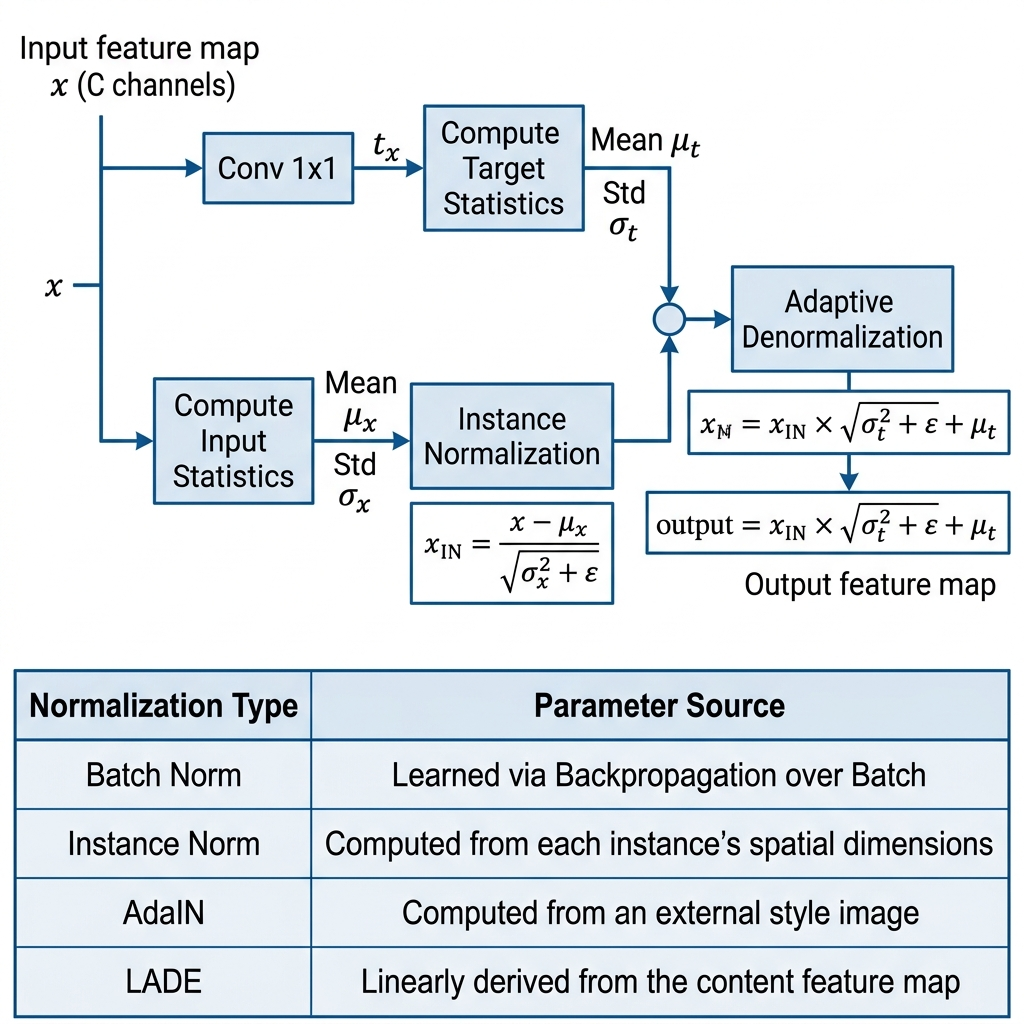
\includegraphics[width=0.88\textwidth]{figChap2/lade_normalization.png}
    \caption{Cơ chế hoạt động của LADE}
    \label{fig:lade}
\end{figure}
    \noindent\textit{Chú thích:} feature map $x$ được chiếu qua Conv $1\times 1$ để tạo thống kê thích ứng $(\mu_t, \sigma_t)$, sau đó bình thường hóa Instance rồi tái tỷ lệ hóa thích ứng. Bảng so sánh cho thấy LADE tự học tham số từ chính dữ liệu, không cần ảnh phong cách riêng như AdaIN \cite{Liu2024}

\subsection{Diễn giải bổ sung và phân tích chi phí}
\label{subsec:lade_analysis}

\textbf{Trường hợp suy biến.} Nếu ma trận trọng số của $\text{Conv}_{1\times1}$ là ma trận đơn vị thì $t_x = x$, kéo theo $\mu_t = \mu_x$, $\sigma_t = \sigma_x$ và do đó $\text{LADE}(x) = x$. Nói cách khác, \textbf{phép đồng nhất nằm trong không gian nghiệm của LADE}. Đây là tính chất quan trọng về mặt tối ưu hóa: mạng luôn có sẵn phương án ``không làm gì'' và chỉ lệch khỏi phương án đó khi việc điều chỉnh phong cách thực sự làm giảm hàm mất mát. Tính chất này giúp huấn luyện ổn định hơn so với các lớp chuẩn hóa mà giá trị khởi tạo ngẫu nhiên bắt buộc phải làm biến dạng đặc trưng.

\textbf{Chi phí tham số.} Mỗi lớp LADE bổ sung một ma trận $C \times C$, tức $C^2$ tham số. Với các lớp trong DTGAN có $C \in \{32, 64, 128\}$, chi phí tương ứng là $1.024$, $4.096$ và $16.384$ tham số --- rất nhỏ so với một lớp tích chập $3\times3$ cùng số kênh ($9C^2$ tham số). Tỉ lệ chi phí phụ trội xấp xỉ:

\begin{equation}
\label{eq:lade_cost}
\frac{\text{tham số LADE}}{\text{tham số Conv}_{3\times3}} = \frac{C^2}{9\,C^2} \approx 11{,}1\%
\end{equation}

\textbf{Chi phí tính toán.} Ngoài tích chập $1\times1$, LADE cần hai lần tính moments trên trục $[H, W]$ --- các phép thu gọn (reduction) có độ phức tạp $O(BHWC)$, tuyến tính theo kích thước tensor và được tối ưu tốt trên GPU. Trên thực tế, phần tốn kém hơn là hai lần duyệt bộ nhớ để tính trung bình rồi phương sai, chứ không phải số phép nhân.

\subsection{So sánh LADE với các kỹ thuật chuẩn hóa khác}
\label{subsec:lade_comparison}

\begin{table}[H]
\caption{So sánh các kỹ thuật chuẩn hóa trong mạng chuyển đổi phong cách ảnh}
\label{tab:norm_comparison}
\centering
\begin{tabular}{|p{2.6cm}|p{3.4cm}|p{3.4cm}|p{3.4cm}|}
\hline
\textbf{Kỹ thuật} & \textbf{Nguồn tham số $(\gamma,\beta)$} & \textbf{Ưu điểm} & \textbf{Hạn chế} \\
\hline
Batch Norm \cite{Ioffe2015} & Thống kê batch & Ổn định huấn luyện & Phụ thuộc batch size \\
\hline
Instance Norm \cite{Ulyanov2016} & Tham số học, cố định & Tốt cho style transfer & Không thích ứng theo ảnh \\
\hline
AdaIN & Từ ảnh phong cách riêng & Linh hoạt phong cách & Cần ảnh style ở suy luận \\
\hline
\textbf{LADE} \cite{Liu2024} & \textbf{Conv $1\times 1$ trên chính $x$} & \textbf{Tự thích ứng theo từng ảnh, không cần style riêng} & \textbf{Tăng $C^2$ tham số mỗi lớp} \\
\hline
\end{tabular}
\end{table}

Sự khác biệt mấu chốt của LADE so với AdaIN là: \textit{tham số tái tỷ lệ hóa được suy ra từ chính feature map hiện tại}, không phải từ một ảnh phong cách bên ngoài. Nhờ đó, mô hình có thể học phong cách nội tại của không gian đặc trưng một cách linh hoạt trong từng bước huấn luyện, và ở giai đoạn suy luận chỉ cần một đầu vào duy nhất --- điều kiện bắt buộc để xuất mô hình sang ONNX với đồ thị tính toán tĩnh.

\subsection{Biến thể LADE\_D trong Discriminator}
\label{subsec:lade_d}

Trong các lớp Discriminator, LADE được mở rộng thành \texttt{LADE\_D}: tích chập $1 \times 1$ trong bước chiếu tuyến tính được thay thế bằng \texttt{spectral\_norm(Conv $1\times1$)} --- tức là áp dụng thêm Spectral Normalization \cite{Miyato2018} để đảm bảo ràng buộc Lipschitz của Discriminator.

Lý do của biến thể này bắt nguồn từ phân tích ở Chương~1 (Mục~\ref{subsec:gan_challenges}): nếu Discriminator có hằng số Lipschitz không bị chặn, nó có thể tạo ra gradient rất lớn và biến động mạnh, đẩy quá trình huấn luyện vào trạng thái không hội tụ. Spectral Normalization chia ma trận trọng số cho giá trị kỳ dị lớn nhất:

\begin{equation}
\label{eq:spectral_norm}
\overline{W}_{\text{SN}} = \frac{W}{\sigma(W)}, \qquad \sigma(W) = \max_{\|h\|_2 \neq 0} \frac{\|W h\|_2}{\|h\|_2}
\end{equation}

\noindent qua đó ràng buộc $\|\overline{W}_{\text{SN}}\|_2 = 1$ và làm cho toàn mạng có hằng số Lipschitz bị chặn.

\medskip
\noindent\textit{\textbf{Nhận xét:} Việc áp Spectral Normalization lên \textit{chính lớp chiếu bên trong LADE} --- chứ không chỉ lên các tích chập chính --- là một chi tiết dễ bị bỏ qua nhưng có logic rõ ràng. Trong LADE, đầu ra của lớp chiếu quyết định hệ số nhân $\sqrt{\sigma_t^2 + \varepsilon}$; nếu hệ số này không bị kiểm soát, một lớp chuẩn hóa hoàn toàn có thể khuếch đại đặc trưng lên nhiều lần và phá vỡ ràng buộc Lipschitz mà các lớp tích chập đã cẩn thận duy trì. Nói cách khác, chuẩn hóa phổ chỉ có ý nghĩa khi được áp \textbf{nhất quán trên mọi đường truyền tín hiệu}, kể cả những đường ``phụ'' nằm trong lớp chuẩn hóa. Theo quan điểm của luận văn, đây là ví dụ điển hình cho thấy chất lượng của một kiến trúc GAN thường nằm ở các chi tiết kỹ thuật nhỏ như vậy, chứ không chỉ ở sơ đồ khối tổng thể.}

% =====================================================
\section{Cơ chế External Attention v3}
\label{sec:external_attention}

\subsection{Hạn chế của Self-Attention và Giải pháp}
\label{subsec:attention_motivation}

Cơ chế Self-Attention \cite{Zhang2019} đã được chứng minh hiệu quả trong việc nắm bắt phụ thuộc tầm xa (long-range dependency) trong ảnh --- khả năng để một pixel ``nhìn thấy'' và tham chiếu tới mọi pixel khác, thay vì chỉ vùng lân cận như tích chập. Trong bài toán anime hóa, khả năng này rất cần thiết: màu tóc ở đỉnh đầu phải nhất quán với màu tóc ở gáy, tông sáng của má trái phải hài hòa với má phải.

Tuy nhiên, Self-Attention tính ma trận tương quan giữa mọi cặp vị trí:

\begin{equation}
\label{eq:self_attention}
\text{SelfAttn}(\mathcal{F}) = \text{Softmax}\!\left(\frac{Q K^{\top}}{\sqrt{d}}\right) V, \qquad Q, K, V \in \mathbb{R}^{N \times C}
\end{equation}

\noindent trong đó $N = H \times W$ là số vị trí không gian. Ma trận $QK^{\top}$ có kích thước $N \times N$, dẫn đến độ phức tạp:

\begin{equation}
\label{eq:self_attn_complexity}
\mathcal{O}(N^2 C) \quad \text{về thời gian}, \qquad \mathcal{O}(N^2) \quad \text{về bộ nhớ}
\end{equation}

Với bottleneck $32 \times 32$ của DTGAN, $N = 1024$ và ma trận attention có $1024^2 \approx 1{,}05$ triệu phần tử --- vẫn chấp nhận được. Nhưng nếu áp dụng ở độ phân giải $64\times64$ thì $N = 4096$ và số phần tử tăng lên $\approx 16{,}8$ triệu, gấp 16 lần. Chính đặc tính tăng trưởng bậc hai này khiến Self-Attention trở thành nút thắt cổ chai khi mở rộng độ phân giải.

External Attention, được đề xuất bởi Guo et al. \cite{Guo2021}, giải quyết vấn đề bằng cách thay thế cặp key--value \textit{nội tại} (sinh từ chính ảnh) bằng hai \textbf{bộ nhớ học được} (learnable memory bank) $M_k$ và $M_v$ \textit{dùng chung cho toàn bộ tập dữ liệu}, giảm độ phức tạp xuống còn $\mathcal{O}(N k C)$ với $k \ll N$.

\subsection{Kiến trúc External Attention v3}
\label{subsec:ext_attention_arch}

\begin{figure}[H]
    \centering
    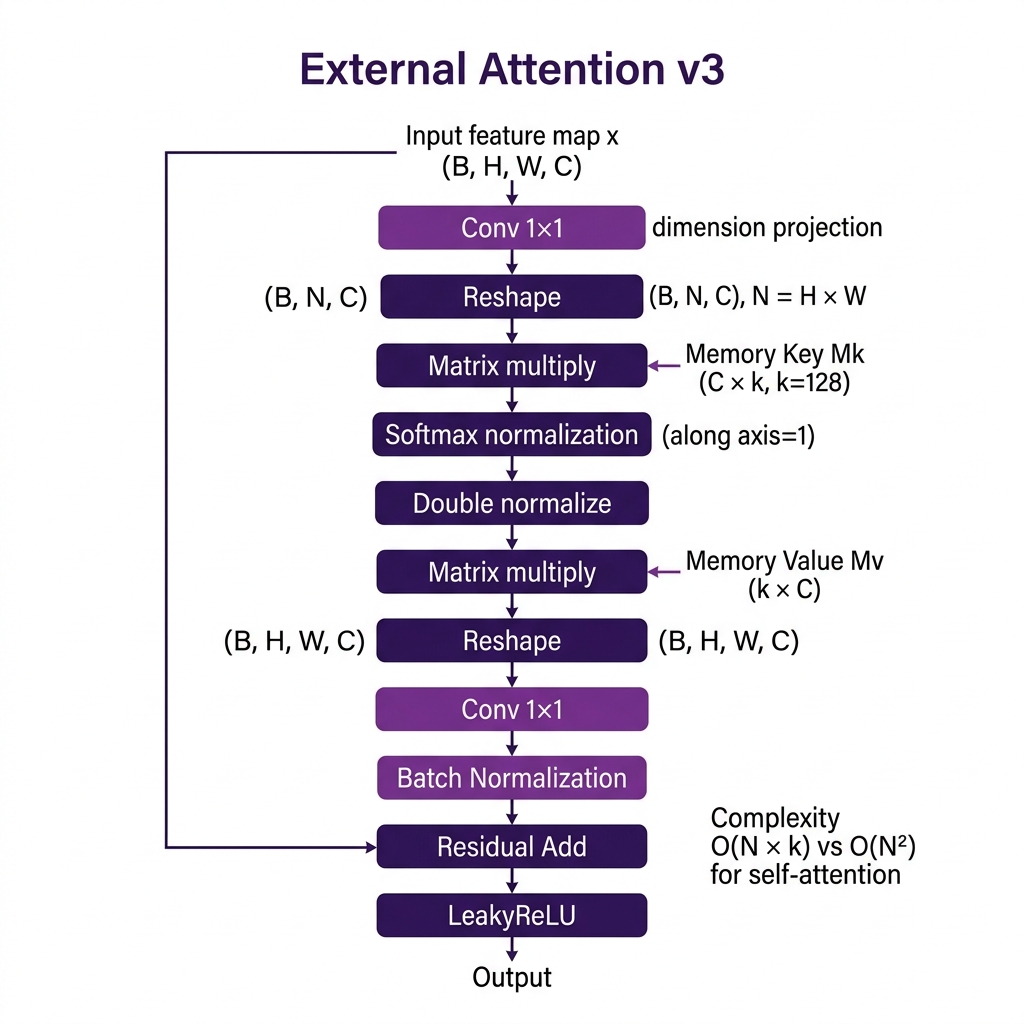
\includegraphics[width=0.68\textwidth]{figChap2/external_attention.png}
    \caption{Kiến trúc External Attention v3 sử dụng trong DTGAN tại vị trí bottleneck $32 \times 32$}
    \label{fig:external_attention}
\end{figure}
    \noindent\textit{Chú thích:} Hai memory bank học được $M_k \in \mathbb{R}^{C \times k}$ và $M_v \in \mathbb{R}^{k \times C}$ cho phép mô hình học phụ thuộc toàn cục với độ phức tạp $O(N \cdot k)$ thay vì $O(N^2)$ của Self-Attention \cite{Guo2021, Liu2024}.

Cụ thể, External Attention v3 trong DTGAN hoạt động theo các bước sau (áp dụng tại bottleneck $32 \times 32$, $k = 128$):

\begin{enumerate}
    \item $x \in \mathbb{R}^{B \times H \times W \times C} \xrightarrow{\text{Conv}_{1\times 1}} $ reshape thành $\mathcal{F} \in \mathbb{R}^{B \times N \times C}$, $N = H \times W$
    \item \textbf{Attention weights:} $A = \text{Softmax}_{\text{axis}=1}\!\left(\mathcal{F} \cdot M_k\right) \in \mathbb{R}^{B \times N \times k}$
    \item \textbf{Double normalization:} $A_{ij} \leftarrow A_{ij} \big/ \sum_j A_{ij}$ (chuẩn hóa theo trục thứ hai)
    \item $\mathcal{F'} = A \cdot M_v \in \mathbb{R}^{B \times N \times C}$, reshape về $\mathbb{R}^{B \times H \times W \times C}$
    \item $\text{out} = \text{LeakyReLU}\!\left(x + \text{BN}\!\left(\text{Conv}_{1\times 1}(\mathcal{F'})\right)\right)$
\end{enumerate}

Công thức tổng quát:
\begin{equation}
\label{eq:ext_attn}
\text{ExternalAttention}(x) = \text{LeakyReLU}\!\left(x + \text{BN}\!\left(\text{normalize}\!\left(\mathcal{F} M_k\right) M_v\right)\right)
\end{equation}

\noindent trong đó:
\begin{itemize}
    \item $\mathcal{F} \in \mathbb{R}^{N \times C}$ --- đặc trưng đã được làm phẳng theo không gian, mỗi hàng là vector đặc trưng $C$ chiều của một vị trí pixel.
    \item $M_k \in \mathbb{R}^{C \times k}$ --- \textit{bộ nhớ khóa}, gồm $k$ vector mẫu (prototype) trong không gian đặc trưng. Đây là tham số học được, \textbf{không phụ thuộc ảnh đầu vào}.
    \item $M_v \in \mathbb{R}^{k \times C}$ --- \textit{bộ nhớ giá trị}, gồm $k$ vector đặc trưng đầu ra tương ứng với từng mẫu.
    \item $A \in \mathbb{R}^{N \times k}$ --- ma trận trọng số chú ý; phần tử $A_{ij}$ thể hiện mức độ pixel thứ $i$ ``thuộc về'' mẫu thứ $j$.
    \item $k = 128$ --- số lượng mẫu trong bộ nhớ, đóng vai trò siêu tham số điều tiết dung lượng biểu diễn.
\end{itemize}

\textbf{Ý nghĩa từng bước:}
\begin{itemize}
    \item \textbf{Bước 2 --- so khớp với từ điển mẫu:} Tích $\mathcal{F} M_k$ tính độ tương đồng giữa mỗi pixel và mỗi vector mẫu. Softmax theo trục $N$ (trục pixel) trả lời câu hỏi: ``\textit{trong toàn bộ ảnh, những pixel nào đại diện tốt nhất cho mẫu $j$?}''. Đây là điểm khác biệt căn bản so với Self-Attention: pixel không so sánh trực tiếp với pixel, mà cùng tham chiếu tới một tập mẫu chung.
    \item \textbf{Bước 4 --- tái tổ hợp:} Tích $A M_v$ tái tạo đặc trưng cho mỗi pixel bằng tổ hợp có trọng số của $k$ vector giá trị. Do $M_v$ dùng chung cho mọi ảnh, các pixel có ngữ nghĩa tương tự (cùng là ``vùng da'', cùng là ``đường viền tóc'') sẽ nhận đặc trưng đầu ra tương tự --- \textbf{đây chính là cơ chế tạo ra tính nhất quán phong cách trên toàn ảnh và trên toàn tập dữ liệu}.
    \item \textbf{Bước 5 --- kết nối dư (residual):} Cộng $x$ vào kết quả đảm bảo module có thể suy biến về phép đồng nhất nếu attention không hữu ích, tương tự tính chất đã phân tích ở Mục~\ref{subsec:lade_analysis}.
\end{itemize}

\subsection{Cơ chế Double Normalization}
\label{subsec:double_norm}

Điểm cải tiến đặc trưng của phiên bản v3 là chuẩn hóa \textbf{hai lần} trên ma trận $A$ theo hai trục khác nhau:

\begin{equation}
\label{eq:double_norm}
\widetilde{A}_{ij} = \frac{\exp(\alpha_{ij})}{\sum_{i'=1}^{N} \exp(\alpha_{i'j})} \quad \text{(chuẩn hóa theo trục pixel)}, \qquad
\widehat{A}_{ij} = \frac{\widetilde{A}_{ij}}{\sum_{j'=1}^{k} \widetilde{A}_{ij'}} \quad \text{(chuẩn hóa theo trục mẫu)}
\end{equation}

\noindent với $\alpha = \mathcal{F} M_k$ là điểm tương đồng thô.

\textbf{Vì sao cần bước thứ hai?} Sau bước softmax theo trục pixel, mỗi \textit{cột} của $A$ có tổng bằng 1, nhưng mỗi \textit{hàng} thì không. Điều này dẫn tới hai vấn đề:

\begin{itemize}
    \item Một pixel có thể có tổng trọng số rất lớn (nếu nó tương đồng cao với nhiều mẫu), làm đặc trưng đầu ra của nó bị khuếch đại bất thường so với các pixel khác --- sinh ra đốm sáng hoặc vệt màu trong ảnh kết quả.
    \item Ngược lại, một số mẫu trong bộ nhớ có thể ``thống trị'' toàn bộ ảnh, khiến các mẫu còn lại không nhận được gradient và dần trở nên vô dụng --- hiện tượng tương tự \textit{sụp đổ mã} (codebook collapse) trong các mô hình lượng tử hóa vector.
\end{itemize}

Bước chuẩn hóa thứ hai buộc tổng trọng số của mỗi pixel bằng 1, biến $\widehat{A}$ thành \textbf{ma trận tổ hợp lồi}: mỗi pixel đầu ra là một trung bình có trọng số của các vector trong $M_v$, không thể vượt ra ngoài bao lồi của chúng. Tính chất này chặn biên độ đầu ra một cách tự nhiên và phân bổ gradient đều hơn cho toàn bộ bộ nhớ.

\subsection{Phân tích độ phức tạp}
\label{subsec:ea_complexity}

\begin{table}[H]
\caption{So sánh độ phức tạp giữa Self-Attention và External Attention tại bottleneck $32\times32$ ($N = 1024$, $C = 128$, $k = 128$)}
\label{tab:attention_complexity}
\centering
\begin{tabular}{|l|c|c|c|}
\hline
\textbf{Cơ chế} & \textbf{Thời gian} & \textbf{Bộ nhớ ma trận attention} & \textbf{Tham số bổ sung} \\
\hline
Self-Attention \cite{Zhang2019} & $\mathcal{O}(N^2 C)$ & $N^2 = 1.048.576$ & $3C^2$ (cho $Q,K,V$) \\
\hline
External Attention \cite{Guo2021} & $\mathcal{O}(N k C)$ & $N k = 131.072$ & $2Ck$ (cho $M_k, M_v$) \\
\hline
\textbf{Tỉ lệ} & $k/N = 1/8$ & \textbf{giảm $8\times$} & \textbf{giảm $\approx 1{,}5\times$} \\
\hline
\end{tabular}
\end{table}

Cần lưu ý rằng mức tiết kiệm phụ thuộc vào tỉ số $k/N$. Tại $32\times32$ với $k=128$, tỉ số này là $1/8$ --- lợi ích rõ nhưng chưa quá lớn. Lợi thế thực sự bộc lộ khi độ phân giải tăng: tại $64\times64$ ($N = 4096$), tỉ số trở thành $1/32$, và tại $128\times128$ là $1/128$. Nói cách khác, chi phí Self-Attention tăng bậc hai còn External Attention tăng \textit{tuyến tính} theo số pixel.

\medskip
\noindent\textit{\textbf{Nhận xét:} Nếu nhìn External Attention qua lăng kính đại số tuyến tính, nó chính là một phép \textbf{xấp xỉ hạng thấp} (low-rank approximation) của ma trận attention: thay vì ma trận $N \times N$ hạng đầy đủ, ta phân tích thành tích của hai ma trận $N \times k$ và $k \times N$ với $k \ll N$. Điều này đồng nghĩa với một sự đánh đổi rõ ràng: mô hình \textbf{mất khả năng biểu diễn các quan hệ pixel--pixel tùy ý}, đổi lại chi phí tuyến tính. Với bài toán tổng quát, đây có thể là mất mát đáng kể; nhưng với bài toán anime hóa, luận văn cho rằng đánh đổi này gần như miễn phí --- vì thứ mà mô hình cần học không phải là quan hệ giữa từng cặp pixel cụ thể, mà là một \textbf{từ điển các loại vùng ảnh} (da, tóc, mắt, nền, viền) và cách tô màu tương ứng cho mỗi loại. Bộ nhớ ngoài $M_k, M_v$ chính là hiện thân trực tiếp của từ điển đó. Đây là một ví dụ tốt cho nguyên tắc: cơ chế đơn giản hơn nhưng \textbf{khớp với cấu trúc của bài toán} thường thắng cơ chế tổng quát hơn nhưng tốn kém.}

% =====================================================
\section{Discriminator (D\_net)}
\label{sec:discriminator}

DTGAN sử dụng hai Discriminator độc lập theo kiến trúc PatchGAN \cite{Isola2017}, mỗi mạng phục vụ một nhánh Generator:

\begin{itemize}
    \item \textbf{Discriminator hỗ trợ (Support D):} Hoạt động trên ảnh xám một kênh. Mạng phân biệt giữa ảnh anime thật đã chuyển sang grayscale và ảnh $\widehat{y}$ (\texttt{generated}) --- sản phẩm của Support Tail sau khi qua Guided Filter. Việc loại bỏ thông tin màu ở đầu vào khiến Discriminator chỉ có thể căn cứ vào cấu trúc hình khối, tương phản sáng tối và hệ thống đường viền để đưa ra phán quyết. Hệ quả là tín hiệu gradient truyền ngược về Support Tail chỉ mang thông tin về các đặc trưng này, buộc nhánh tập trung học đường nét thay vì màu sắc.
    \item \textbf{Discriminator chính (Main D):} Hoạt động trên ảnh màu ba kênh (RGB). Mạng phân biệt giữa ảnh anime thật đã tiền xử lý bằng NL-Means kết hợp L0 Smoothing và ảnh màu $\widehat{y}_m$ do Main Tail sinh ra. Do đầu vào giữ đầy đủ thông tin màu, Discriminator có thể phát hiện các sai lệch về phối màu, độ bão hòa và tính đồng nhất của các mảng màu --- những yếu tố quyết định hiệu ứng cel-shading. Việc đối chiếu với ảnh anime đã khử nhiễu hạt giúp tín hiệu học tập trung vào phân bố màu theo vùng thay vì kết cấu bề mặt chi tiết.
\end{itemize}

Mỗi Discriminator gồm 7 lớp tích chập sử dụng \texttt{LADE\_D} (LADE kết hợp Spectral Normalization), đầu ra là feature map một kênh theo phong cách PatchGAN.

\textbf{Nguyên lý PatchGAN.} Khác với Discriminator truyền thống trả về một số vô hướng cho toàn ảnh, PatchGAN trả về một bản đồ điểm số $D(\cdot) \in \mathbb{R}^{H' \times W'}$, trong đó mỗi phần tử đánh giá một vùng cục bộ của ảnh:

\begin{equation}
\label{eq:patchgan}
\mathcal{L}_{\text{patch}} = \frac{1}{H' W'} \sum_{u=1}^{H'} \sum_{v=1}^{W'} \ell\big(D(\cdot)_{u,v}\big)
\end{equation}

\noindent trong đó $\ell(\cdot)$ là hàm mất mát điểm (ở DTGAN là bình phương sai lệch của LSGAN), và mỗi vị trí $(u,v)$ có trường tiếp nhận tương ứng với một vùng ảnh gốc kích thước cố định. Thiết kế này có ba lợi ích trực tiếp cho bài toán anime hóa:

\begin{enumerate}
    \item \textbf{Tín hiệu học dày đặc hơn:} thay vì một tín hiệu cho cả ảnh, Generator nhận $H' \times W'$ tín hiệu, giúp gradient giàu thông tin không gian và hội tụ nhanh hơn.
    \item \textbf{Tập trung vào kết cấu cục bộ:} phong cách anime được xác định chủ yếu bởi đặc tính cục bộ (nét viền, mảng màu), không phải bố cục toàn cục --- vốn phải được giữ nguyên từ ảnh gốc. PatchGAN vì vậy khớp với bản chất bài toán.
    \item \textbf{Ít tham số hơn:} không cần lớp fully-connected ở cuối, đồng thời cho phép mạng xử lý ảnh ở kích thước tùy ý --- điều kiện cần thiết cho Landscape Mode ở Chương~3, nơi ảnh đầu vào không cố định $256\times256$.
\end{enumerate}

\medskip
\noindent\textit{\textbf{Phân tích thiết kế:} Lựa chọn ép Support Discriminator làm việc trên ảnh xám là một can thiệp mang tính \textbf{ràng buộc thông tin} (information bottleneck) rất đáng chú ý. Thông thường, người thiết kế mạng có xu hướng cung cấp cho mô hình càng nhiều thông tin càng tốt. Ở đây, các tác giả làm ngược lại: chủ động \textit{cắt bỏ} kênh màu để định hướng việc học. Cơ sở của thủ thuật này nằm ở chỗ Discriminator chỉ có thể phạt Generator dựa trên những gì nó \textit{quan sát được} --- nếu nó không thấy màu, nó không thể tạo ra gradient liên quan tới màu. Nói cách khác, \textbf{kiến trúc đầu vào của Discriminator chính là một cách đặc tả hàm mất mát}, và đây là công cụ định hướng học tinh tế hơn nhiều so với việc chỉ điều chỉnh trọng số các số hạng loss. Luận văn cho rằng đây là một trong những ý tưởng có tính chuyển giao cao nhất của DTGAN: nguyên tắc ``giới hạn quan sát của giám khảo để chuyên biệt hóa thí sinh'' có thể áp dụng cho nhiều bài toán sinh ảnh đa mục tiêu khác.}

% =====================================================
\section{Các hàm mất mát được sử dụng trong kiến trúc}
\label{sec:loss}

DTGAN sử dụng một hệ thống hàm mất mát đa thành phần, phản ánh mục tiêu kép của hai nhánh decoder. Hình~\ref{fig:loss_diagram} minh họa toàn bộ pipeline. Mỗi hàm mất mát dưới đây được trình bày theo format thống nhất: \textbf{Tên} $\to$ \textbf{Ý nghĩa/Tác dụng} $\to$ \textbf{Công thức} $\to$ \textbf{Giải thích}.

\begin{figure}[H]
    \centering
    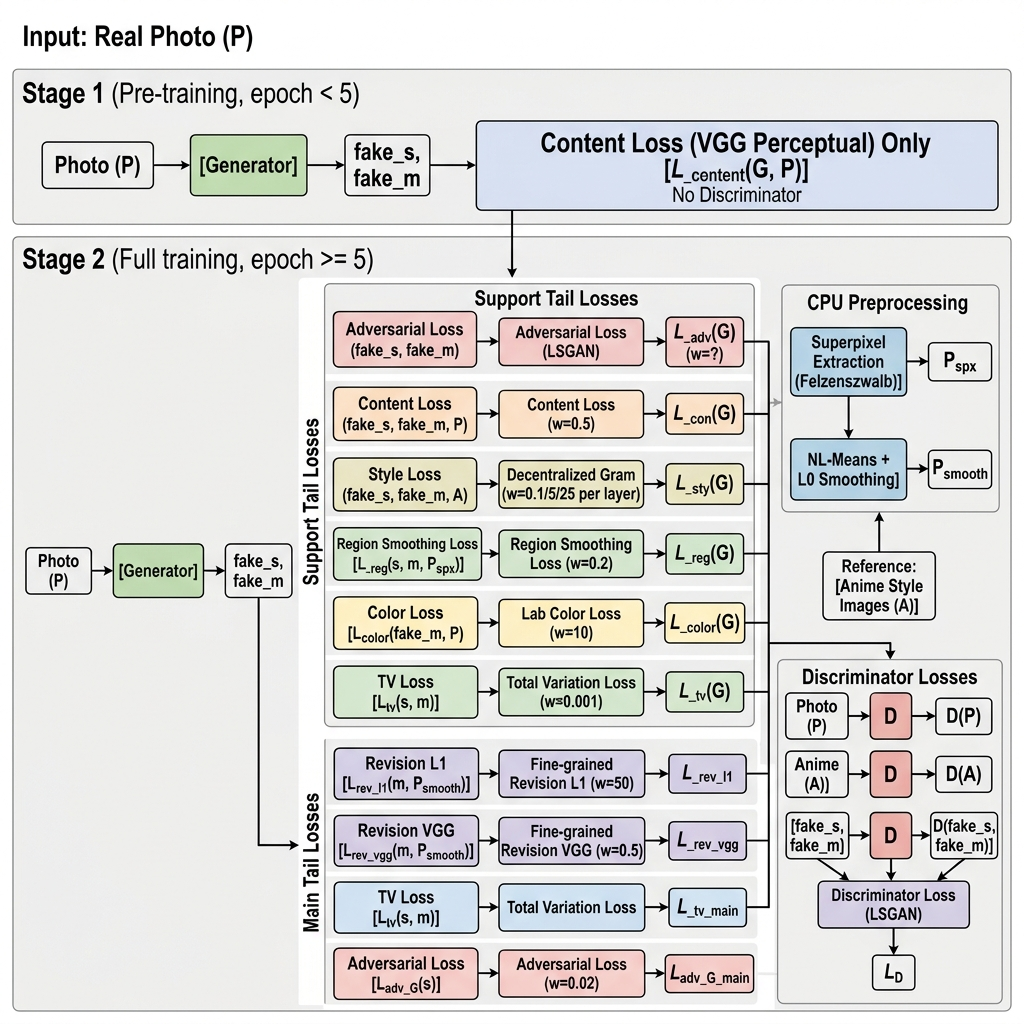
\includegraphics[width=\textwidth]{figChap2/loss_functions_diagram.png}
    \caption{Pipeline huấn luyện hai giai đoạn và hệ thống hàm mất mát của DTGAN}
    \label{fig:loss_diagram}
\end{figure}
    \noindent\textit{Chú thích:} Giai đoạn 1 (pre-training) chỉ dùng Content Loss. Giai đoạn 2 kết hợp nhiều thành phần loss cho Support Tail và Main Tail, với pseudo ground-truth được tạo bởi CPU preprocessing \cite{Liu2024}

\subsection{Tổng quan hệ thống hàm mất mát}
\label{subsec:loss_overview}

Trước khi đi vào từng thành phần, Bảng~\ref{tab:loss_summary} tổng hợp toàn bộ hệ thống để tiện đối chiếu. Mỗi hàm mất mát trả lời một câu hỏi khác nhau về chất lượng ảnh sinh ra.

\begin{table}[H]
\caption{Tổng hợp hệ thống hàm mất mát của DTGAN}
\label{tab:loss_summary}
\centering
\fontsize{11}{13}\selectfont
\begin{tabular}{|p{2.6cm}|p{4.3cm}|p{2.5cm}|p{3.6cm}|}
\hline
\textbf{Hàm mất mát} & \textbf{Câu hỏi cần trả lời} & \textbf{Áp dụng cho} & \textbf{Trọng số} \\
\hline
Content $\mathcal{L}_{\text{con}}$ & Ảnh sinh có giữ đúng nội dung gốc? & Cả hai nhánh & $\lambda_{\text{con}}$ \\
\hline
Style $\mathcal{L}_{\text{sty}}$ & Kết cấu có giống phong cách anime? & Support Tail & $(0{,}1;\ 5{,}0;\ 25{,}0)$ theo tầng \\
\hline
Region Smoothing $\mathcal{L}_{\text{rs}}$ & Vùng màu đã đủ phẳng? & Support Tail & $0{,}2$ mỗi số hạng \\
\hline
Lab Color $\mathcal{L}_{\text{color}}$ & Màu có bị trôi khỏi ảnh gốc? & Support Tail & $\lambda_{\text{col}} = 10{,}0$ \\
\hline
Total Variation $\mathcal{L}_{\text{TV}}$ & Ảnh có nhiễu pixel cục bộ? & Cả hai nhánh & $\lambda_{\text{TV}} = 0{,}001$ \\
\hline
Adversarial $\mathcal{L}_{\text{adv}}$ & Discriminator có bị đánh lừa? & Cả hai nhánh & $1{,}0$ (S) / $0{,}02$ (M) \\
\hline
Revision $\mathcal{L}_{\text{rev}}$ & Có bám sát pseudo ground-truth? & Main Tail & $\lambda_{r1}=50{,}0$; $\lambda_{rv}=0{,}5$ \\
\hline
\end{tabular}
\end{table}

% GHI CHÚ: giá trị lambda_con cần được điền theo file cấu hình huấn luyện thực tế của bạn.

\subsection{Hàm mất mát Giai đoạn Pre-training}
\label{subsec:pretrain_loss}

Trong các epoch đầu ($\text{epoch} < \text{init\_G\_epoch} = 5$), chỉ huấn luyện Generator với Content Loss thuần túy (không có Discriminator):

\begin{equation}
\label{eq:pretrain_loss}
\mathcal{L}_{\text{pre}} = \mathcal{L}_{\text{con}}(x, \widehat{y}_s) + \mathcal{L}_{\text{con}}(x, \widehat{y}_m)
\end{equation}

Ở giai đoạn này, mục tiêu duy nhất là để cả hai nhánh học tái tạo ảnh đầu vào ở mức đặc trưng ngữ nghĩa --- nói cách khác, Generator được huấn luyện như một \textbf{bộ tự mã hóa} (autoencoder). Điều này giải quyết một vấn đề cụ thể trong huấn luyện GAN: nếu kích hoạt tín hiệu đối kháng ngay từ bước đầu, Generator (với trọng số khởi tạo ngẫu nhiên) sinh ra ảnh nhiễu hoàn toàn, Discriminator phân biệt được ngay lập tức với độ chính xác gần 100\%, và như đã phân tích ở Chương~1 (Mục~\ref{subsec:gan_challenges}), gradient truyền về Generator trở nên rất nhỏ --- hiện tượng biến mất gradient ở giai đoạn đầu.

\subsection{Content Loss (Perceptual Loss)}
\label{subsec:content_loss}

Content Loss được tính thông qua mạng VGG19 \cite{Simonyan2015} tại lớp \texttt{conv4\_4} (512 kênh):

\begin{equation}
\label{eq:content_loss}
\mathcal{L}_{\text{con}}(x, \widehat{y}) = \frac{1}{C_l H_l W_l} \left\| \phi_l(x) - \phi_l(\widehat{y}) \right\|_1
\end{equation}

\noindent trong đó:
\begin{itemize}
    \item $\phi_l(\cdot)$ --- ánh xạ trích xuất đặc trưng tại lớp $l$ của mạng VGG19 đã huấn luyện sẵn trên ImageNet; trọng số VGG được \textbf{đóng băng}, không cập nhật trong quá trình huấn luyện.
    \item $C_l, H_l, W_l$ --- số kênh, chiều cao, chiều rộng của bản đồ đặc trưng tại lớp $l$; tích của chúng dùng để chuẩn hóa, giúp giá trị loss không phụ thuộc kích thước tầng.
    \item $\|\cdot\|_1$ --- chuẩn $L_1$ (tổng trị tuyệt đối của các sai lệch).
\end{itemize}

\textbf{Vì sao so sánh ở không gian đặc trưng thay vì không gian pixel?} Nếu dùng $\|x - \widehat{y}\|_1$ trực tiếp trên pixel, hàm mất mát sẽ phạt \textit{mọi} thay đổi --- bao gồm cả những thay đổi mà ta \textit{mong muốn} (làm phẳng màu, đơn giản hóa kết cấu). Kết quả là ảnh đầu ra sẽ gần như trùng ảnh gốc và không hề mang phong cách anime. Ngược lại, đặc trưng tại tầng sâu như \texttt{conv4\_4} mã hóa thông tin ngữ nghĩa (``đây là mắt'', ``đây là đường viền mặt'') và tương đối bất biến với thay đổi màu sắc, kết cấu bề mặt. Do đó $\mathcal{L}_{\text{con}}$ ràng buộc ``\textit{vẫn là khuôn mặt đó}'' mà không ràng buộc ``\textit{vẫn là những pixel đó}''.

\textbf{Vì sao chọn tầng \texttt{conv4\_4}?} Đây là điểm cân bằng: các tầng nông (\texttt{conv1}, \texttt{conv2}) còn mang nhiều thông tin kết cấu và màu, ràng buộc quá chặt; các tầng quá sâu (\texttt{conv5}) trừu tượng đến mức mất thông tin vị trí, khiến ảnh đầu ra có thể biến dạng hình học.

\textbf{Vì sao dùng chuẩn $L_1$ thay vì $L_2$?} Chuẩn $L_2$ phạt bình phương sai lệch nên rất nhạy với các giá trị ngoại lai; nghiệm tối ưu của nó là \textit{trung bình} của các khả năng, dẫn tới hiện tượng ảnh bị mờ khi bài toán có nhiều lời giải hợp lệ (như trường hợp chuyển phong cách). Chuẩn $L_1$ có nghiệm tối ưu là \textit{trung vị}, ít bị kéo bởi ngoại lai và cho ảnh sắc nét hơn \cite{Johnson2016}.

\subsection{Style Loss (Decentralized Gram Matrix)}
\label{subsec:style_loss}

Style Loss là thành phần giúp Generator học phân phối phong cách anime thông qua ma trận Gram. Ý tưởng nền tảng: \textbf{ma trận Gram đo mức độ đồng xuất hiện giữa các kênh đặc trưng}. Nếu kênh ``phát hiện cạnh dọc'' và kênh ``phát hiện màu vàng nhạt'' thường kích hoạt cùng nhau, phần tử Gram tương ứng sẽ lớn --- và đó chính là một đặc điểm phong cách. Quan trọng là phép tính này \textit{tổng hợp trên toàn bộ vị trí không gian}, nên nó nắm bắt ``chất liệu'' của ảnh mà bỏ qua ``ảnh vẽ cái gì''.

Điểm đặc biệt của DTGAN là sử dụng \textbf{Decentralized Gram Matrix} --- trừ đi trung bình của activations trước khi tính Gram:

\begin{equation}
\label{eq:decentralized_gram}
G_l^{\text{dec}}(x) = \frac{1}{C_l N_l} \left(\phi_l(x) - \bar{\phi}_l(x)\right)^{\top} \left(\phi_l(x) - \bar{\phi}_l(x)\right)
\end{equation}

\noindent trong đó $\bar{\phi}_l(x) = \frac{1}{N_l}\sum_{i} \phi_l(x)_i$ là trung bình của activation map tại lớp $l$, và $N_l = H_l W_l$ là số vị trí không gian.

\textbf{Vì sao phải trừ trung bình?} Ma trận Gram cổ điển $\phi^{\top}\phi$ thực chất là \textbf{ma trận moment bậc hai chưa tâm hóa}, nên nó lẫn lộn hai loại thông tin: (i) mức kích hoạt trung bình của từng kênh, và (ii) sự \textit{biến thiên tương quan} giữa các kênh. Với bài toán anime hóa, thành phần (i) chủ yếu phản ánh độ sáng tổng thể --- mà ảnh anime thường sáng và bão hòa hơn hẳn ảnh chụp thật. Nếu không tâm hóa, Style Loss sẽ bị chi phối bởi chênh lệch độ sáng và Generator sẽ ``ăn gian'' bằng cách chỉ tăng độ sáng toàn ảnh thay vì học kết cấu anime thật sự. Sau khi trừ trung bình, $G^{\text{dec}}$ trở thành \textbf{ma trận hiệp phương sai giữa các kênh}, chỉ giữ lại thông tin tương quan --- đúng thứ định nghĩa phong cách.

Loss style tổng hợp từ ba lớp VGG19 (\texttt{conv2\_2}, \texttt{conv3\_4}, \texttt{conv4\_4}) với trọng số tăng dần:

\begin{equation}
\label{eq:style_loss}
\mathcal{L}_{\text{sty}} = \lambda_{s1} \left\|G_2^{\text{dec}}\right\| + \lambda_{s2} \left\|G_3^{\text{dec}}\right\| + \lambda_{s3} \left\|G_4^{\text{dec}}\right\|
\end{equation}

\noindent với $(\lambda_{s1}, \lambda_{s2}, \lambda_{s3}) = (0{,}1;\ 5{,}0;\ 25{,}0)$.

\textbf{Ý nghĩa của bộ trọng số tăng dần.} Chênh lệch $250\times$ giữa tầng nông nhất và tầng sâu nhất không phải ngẫu nhiên. Tầng \texttt{conv2\_2} mã hóa kết cấu vi mô (hạt nhiễu, chi tiết da); nếu đặt trọng số cao, mô hình sẽ sao chép kết cấu vẽ tay ở mức pixel và sinh ra nhiễu dạng hạt. Tầng \texttt{conv4\_4} mã hóa các mô-típ phong cách ở phạm vi rộng (cách xử lý mảng sáng tối, cách nhóm màu) --- đây mới là thứ cần học mạnh. Ngoài ra, giá trị tuyệt đối của Gram tại tầng nông thường lớn hơn nhiều do số kênh ít và activation dày đặc, nên trọng số nhỏ cũng có tác dụng \textbf{cân bằng thang đo} giữa các tầng.

\subsection{Region Smoothing Loss}
\label{subsec:region_loss}

Một trong những đặc trưng quan trọng của phong cách anime là \textbf{các vùng màu phẳng}, tối giản chi tiết kết cấu. Region Smoothing Loss được thiết kế để khuyến khích tính chất này bằng cách sử dụng \textbf{Superpixel Segmentation} (thuật toán Felzenszwalb \cite{Felzenszwalb2004}) để tạo phiên bản ``tối giản'' $x_{\text{spx}}$ của ảnh đầu vào:

\begin{equation}
\label{eq:region_loss}
\mathcal{L}_{\text{rs}} = 0{,}2 \cdot \mathcal{L}_{\text{con}}(x_{\text{spx}},\, \widehat{y}_s) + 0{,}2 \cdot \mathcal{L}_{\text{con}}(x_{\text{spx}},\, \widehat{y})
\end{equation}

\noindent trong đó $\widehat{y}_s$ là đầu ra thô của Support Tail và $\widehat{y}$ là đầu ra sau Guided Filter. Việc ràng buộc \textit{cả hai} phiên bản đảm bảo tính phẳng vùng được duy trì trước và sau khâu lọc, tránh trường hợp Guided Filter phải ``gánh'' toàn bộ nhiệm vụ làm mịn.

\textbf{Cách tạo $x_{\text{spx}}$.} Thuật toán Felzenszwalb phân chia ảnh thành các vùng đồng nhất về màu sắc và cường độ (superpixel) bằng cách xây dựng đồ thị lân cận trên pixel và gộp các vùng có chênh lệch nội vùng nhỏ hơn chênh lệch liên vùng. Sau khi phân vùng, mỗi superpixel được thay thế bằng \textbf{màu trung bình} của vùng đó. Kết quả là một phiên bản ``đã tô phẳng'' của ảnh gốc --- rất gần với hiệu ứng cel-shading, nhưng vẫn giữ nguyên bố cục và ranh giới các đối tượng.

\textbf{Vì sao dùng $\mathcal{L}_{\text{con}}$ (đặc trưng VGG) mà không so sánh pixel trực tiếp?} Nếu buộc ảnh đầu ra trùng khớp $x_{\text{spx}}$ ở mức pixel, mô hình sẽ sao chép luôn các \textit{lỗi phân vùng} của thuật toán Felzenszwalb (biên vùng răng cưa, vùng bị gộp sai). Việc so sánh ở không gian đặc trưng chỉ truyền đạt thông điệp ``\textit{hãy phẳng như thế này}'' mà không áp đặt từng ranh giới cụ thể --- một dạng giám sát mềm.

\textbf{Vì sao trọng số chỉ $0{,}2$?} Đây là số hạng có tính chất ``gợi ý xu hướng'' chứ không phải ràng buộc cứng. Nếu đặt trọng số cao, mô hình sẽ làm phẳng cả những vùng cần giữ chi tiết --- đặc biệt là mắt và tóc trong ảnh chân dung.

\subsection{Lab Color Loss}
\label{subsec:color_loss}

Để bảo toàn màu sắc tự nhiên từ ảnh gốc (tránh hiện tượng trôi màu --- color drift --- trong quá trình chuyển đổi phong cách), DTGAN sử dụng Lab Color Loss trong không gian màu CIE Lab:

\begin{equation}
\label{eq:color_loss}
\mathcal{L}_{\text{color}} = 2 \cdot \left\| L(x) - L(\widehat{y}) \right\|_1 + \left\| a(x) - a(\widehat{y}) \right\|_1 + \left\| b(x) - b(\widehat{y}) \right\|_1
\end{equation}

\noindent trong đó:
\begin{itemize}
    \item $L(\cdot) \in [0, 100]$ --- kênh độ sáng (lightness), $0$ là đen tuyệt đối, $100$ là trắng.
    \item $a(\cdot)$ --- trục màu đối lập xanh lục $\leftrightarrow$ đỏ.
    \item $b(\cdot)$ --- trục màu đối lập xanh lam $\leftrightarrow$ vàng.
\end{itemize}

\textbf{Vì sao là Lab mà không phải RGB?} Trong không gian RGB, ba kênh có tương quan cao và đều mang thông tin độ sáng lẫn sắc độ trộn lẫn --- không thể tách riêng để đặt trọng số. Không gian CIE Lab được thiết kế theo nguyên tắc \textit{đồng đều về cảm nhận} (perceptually uniform): khoảng cách Euclid giữa hai màu trong Lab tỉ lệ xấp xỉ với mức độ khác biệt mà mắt người cảm nhận được. Quan trọng hơn, Lab \textbf{tách bạch độ sáng khỏi sắc độ}, cho phép hàm mất mát ràng buộc hai khía cạnh này với mức độ khác nhau --- đúng nhu cầu của bài toán: giữ chặt cấu trúc sáng--tối (vốn xác định hình khối và danh tính khuôn mặt) nhưng nới lỏng sắc độ (để mô hình được tự do dịch màu theo bảng màu anime).

\textbf{Vì sao kênh $L$ có trọng số gấp đôi?} Sai lệch độ sáng gây biến dạng hình khối và làm thay đổi đặc điểm nhận dạng khuôn mặt, trong khi sai lệch sắc độ ở mức vừa phải lại là điều \textit{mong muốn} khi anime hóa. Hệ số 2 mã hóa chính thứ tự ưu tiên này. Trọng số toàn cục $\lambda_{\text{col}} = 10{,}0$.

\subsection{Total Variation Loss}
\label{subsec:tv_loss}

Total Variation (TV) Loss thúc đẩy tính mịn không gian của ảnh đầu ra, giảm nhiễu pixel cục bộ:

\begin{equation}
\label{eq:tv_loss}
\mathcal{L}_{\text{TV}}(\widehat{y}) = \frac{1}{HW} \sum_{i,j} \left( \left\|\nabla_h \widehat{y}_{i,j}\right\|^2 + \left\|\nabla_w \widehat{y}_{i,j}\right\|^2 \right)
\end{equation}

\noindent trong đó $\nabla_h \widehat{y}_{i,j} = \widehat{y}_{i+1,j} - \widehat{y}_{i,j}$ và $\nabla_w \widehat{y}_{i,j} = \widehat{y}_{i,j+1} - \widehat{y}_{i,j}$ là sai phân hữu hạn theo chiều dọc và chiều ngang --- xấp xỉ rời rạc của gradient ảnh.

Hàm này phạt tổng bình phương biến thiên giữa các pixel kề nhau, do đó khuyến khích ảnh đầu ra ``ít gợn''. Trọng số được đặt rất nhỏ, $\lambda_{\text{TV}} = 0{,}001$, và điều này hoàn toàn có chủ ý: TV Loss về bản chất \textbf{đối kháng với mục tiêu đường nét sắc}. Nếu tăng trọng số, ảnh sẽ mịn nhưng các đường viền anime --- vốn là những vùng gradient lớn --- sẽ bị làm mờ. Vai trò của TV ở đây chỉ là khử các đốm nhiễu đơn lẻ do tích chập sinh ra, chứ không phải làm mịn tổng thể (nhiệm vụ đó đã thuộc về Region Smoothing Loss và Guided Filter).

\subsection{Adversarial Loss (LSGAN)}
\label{subsec:adv_loss}

DTGAN sử dụng biến thể LSGAN (Least Squares GAN) \cite{Mao2017} thay vì hàm mất mát entropy chéo, giúp tránh vấn đề biến mất gradient khi Discriminator hội tụ. Loss cho Generator:
\begin{equation}
\label{eq:gen_adv_loss}
\mathcal{L}_{\text{adv}}^G = \mathbb{E}\!\left[\left(D(\widehat{y}) - 1\right)^2\right]
\end{equation}

Loss cho Discriminator Support:
\begin{equation}
\label{eq:disc_support_loss}
\mathcal{L}_D^s = \underbrace{\mathbb{E}\!\left[\left(D(y_{\text{anime}}) - 1\right)^2\right]}_{\text{(1) ảnh anime thật} \to 1} + \underbrace{\mathbb{E}\!\left[D(\widehat{y})^2\right]}_{\text{(2) ảnh sinh} \to 0} + \underbrace{2{,}0 \cdot \mathbb{E}\!\left[D(y_{\text{smooth}})^2\right]}_{\text{(3) ảnh anime mờ nét} \to 0}
\end{equation}

\noindent trong đó $y_{\text{anime}}$ là ảnh anime thật, $\widehat{y}$ là ảnh do Generator sinh ra, và $y_{\text{smooth}}$ là ảnh anime đã được làm mờ vùng biên (edge-smoothed).

\textbf{Ý nghĩa từng số hạng:}
\begin{itemize}
    \item \textbf{Số hạng (1) và (2)} là cặp đối kháng chuẩn: Discriminator học gán điểm 1 cho ảnh thật và 0 cho ảnh giả.
    \item \textbf{Số hạng (3)} là điểm đặc sắc kế thừa từ CartoonGAN \cite{Chen2018CartoonGAN}. Tập $y_{\text{smooth}}$ được tạo bằng cách lấy chính ảnh anime thật rồi làm mờ riêng vùng biên. Ảnh này giống ảnh anime thật ở mọi phương diện --- màu sắc, bố cục, phân bố vùng --- \textbf{ngoại trừ độ sắc của đường nét}. Bằng cách buộc Discriminator gán điểm 0 cho chúng, ta cô lập được đúng một đặc trưng để phạt: sự thiếu sắc nét ở đường viền. Không có số hạng này, Generator hoàn toàn có thể đạt điểm cao chỉ bằng cách khớp phân bố màu mà bỏ qua đường nét --- đúng nhược điểm thường thấy ở các mô hình anime hóa thế hệ trước.
    \item \textbf{Hệ số $2{,}0$} khiến mức phạt cho ``ảnh mờ nét'' nặng gấp đôi ``ảnh giả thông thường'', phản ánh mức độ ưu tiên của đường nét trong phong cách anime.
\end{itemize}

\textbf{Vì sao chọn LSGAN thay vì entropy chéo hoặc WGAN-GP?} Như đã phân tích ở Chương~1 (Mục~\ref{subsubsec:lsgan} và Mục~\ref{subsubsec:wgan_gp}), hàm entropy chéo bão hòa khi Discriminator quá mạnh: khi $D(\widehat{y}) \to 0$, gradient $\partial \log(1 - D)/\partial D$ trở nên rất nhỏ và Generator ngừng học. LSGAN dùng sai số bình phương, nên gradient tỉ lệ \textit{tuyến tính} với khoảng cách tới mục tiêu --- mẫu càng bị phân loại sai càng nhận gradient lớn, không bao giờ bão hòa. So với WGAN-GP, LSGAN có ưu thế thực tiễn rõ rệt: không cần tính gradient penalty (vốn đòi hỏi đạo hàm bậc hai, làm chậm mỗi bước huấn luyện đáng kể) và không cần huấn luyện Discriminator nhiều bước cho mỗi bước Generator. Với một mô hình hướng tới triển khai nhẹ và huấn luyện được trên một GPU đơn như DTGAN, đây là đánh đổi hợp lý.

\subsection{Fine-grained Revision Loss (Main Tail)}
\label{subsec:revision_loss}

Thành phần loss đặc trưng nhất của Main Tail là \textbf{Fine-grained Revision Loss}, sử dụng pseudo ground-truth $x_{\text{smooth}}$ tạo bởi NL-Means Denoising \cite{Buades2005NLM} kết hợp với L0 Gradient Minimization \cite{Xu2011L0}:

\begin{equation}
\label{eq:revision_loss}
\mathcal{L}_{\text{rev}} = \lambda_{r1} \cdot \left\|x_{\text{smooth}} - \widehat{y}_m\right\|_1 + \lambda_{rv} \cdot \mathcal{L}_{\text{con}}(x_{\text{smooth}}, \widehat{y}_m)
\end{equation}

\noindent với $\lambda_{r1} = 50{,}0$ và $\lambda_{rv} = 0{,}5$.

\textbf{Cách tạo pseudo ground-truth.} Hai bước tiền xử lý bổ trợ cho nhau:
\begin{itemize}
    \item \textbf{NL-Means Denoising} khử nhiễu bằng cách thay mỗi pixel bằng trung bình có trọng số của các pixel có \textit{vùng lân cận tương tự} trên toàn ảnh. Bước này loại bỏ hạt nhiễu cảm biến và kết cấu da mà vẫn giữ cấu trúc.
    \item \textbf{L0 Gradient Minimization} tối thiểu hóa \textit{số lượng} pixel có gradient khác 0 (chuẩn $L_0$), thay vì tổng độ lớn gradient như TV Loss. Hệ quả toán học rất khác biệt: chuẩn $L_1/L_2$ khuyến khích mọi gradient nhỏ lại (làm mờ đều), còn chuẩn $L_0$ khuyến khích \textit{phần lớn} gradient bằng 0 nhưng \textit{cho phép một số ít gradient rất lớn} --- tức là đúng cấu trúc ``vùng phẳng ngăn cách bởi biên sắc'' của tranh anime.
\end{itemize}

\textbf{Ý nghĩa của tỉ lệ trọng số $50{,}0$ so với $0{,}5$.} Chênh lệch $100\times$ cho thấy Main Tail được huấn luyện chủ yếu như một bài toán \textbf{hồi quy có giám sát} chứ không phải sinh ảnh đối kháng. Số hạng $L_1$ trên pixel đảm bảo bám sát chính xác pseudo ground-truth; số hạng perceptual với trọng số nhỏ chỉ đóng vai trò ràng buộc nhất quán ngữ nghĩa, ngăn ảnh trôi khỏi nội dung gốc khi $L_1$ có nhiều nghiệm tương đương. Kết hợp với $\lambda_{\text{adv}}^m = 0{,}02$ ở phần sau, có thể thấy tín hiệu đối kháng đối với Main Tail chỉ mang tính ``điều chỉnh tinh'', chiếm tỉ trọng rất nhỏ.

\subsection{Tổng hợp Loss}
\label{subsec:total_loss}

\begin{align}
\label{eq:total_support_loss}
\mathcal{L}_G^{\text{support}} &= \mathcal{L}_{\text{adv}}^s + \lambda_{\text{con}} \cdot \mathcal{L}_{\text{con}} + \mathcal{L}_{\text{sty}} + \mathcal{L}_{\text{rs}} + \lambda_{\text{col}} \cdot \mathcal{L}_{\text{color}} + \lambda_{\text{TV}} \cdot \mathcal{L}_{\text{TV}}(\widehat{y}) \\
\label{eq:total_main_loss}
\mathcal{L}_G^{\text{main}} &= \lambda_{\text{adv}}^m \cdot \mathcal{L}_{\text{adv}}^m + \mathcal{L}_{\text{rev}} + \lambda_{\text{TV}} \cdot \mathcal{L}_{\text{TV}}(\widehat{y}_m)
\end{align}

Tổng loss Generator: $\mathcal{L}_G = \mathcal{L}_G^{\text{support}} + \mathcal{L}_G^{\text{main}}$, với $\lambda_{\text{adv}}^m = 0{,}02$.

\medskip
\noindent\textit{\textbf{Thảo luận về cân bằng trọng số:} Hệ thống bảy hàm mất mát với các trọng số trải trên năm bậc độ lớn --- từ $0{,}001$ (TV) đến $50{,}0$ (Revision $L_1$) --- là điểm vừa mạnh vừa mong manh nhất của DTGAN. Mạnh, vì mỗi số hạng phụ trách đúng một khía cạnh chất lượng và có thể điều chỉnh độc lập. Mong manh, vì bộ trọng số này gắn chặt với đặc điểm của tập dữ liệu huấn luyện. Kết quả thực nghiệm ở Chương~4 minh họa rõ điều này: các thành phần loss ổn định ở những mức rất khác nhau (style $\approx 3{,}42$; color $\approx 0{,}67$; content $\approx 0{,}19$; region smoothing $\approx 0{,}20$), nghĩa là chúng \textbf{không đóng góp ngang nhau} vào gradient tổng --- Style Loss chi phối phần lớn tín hiệu học. Một hệ quả thực tiễn quan trọng: khi chuyển sang tập phong cách khác (ví dụ từ Hayao sang Shinkai với tông màu và độ tương phản rất khác), bộ trọng số tối ưu nhiều khả năng cũng phải thay đổi. Theo quan điểm của luận văn, đây là một hạn chế nội tại của các phương pháp dựa trên tổ hợp tuyến tính nhiều hàm mất mát, và là lý do khiến việc \textbf{mở rộng sang mô hình đa phong cách} (đề xuất ở Chương~5) không thể chỉ đơn thuần là huấn luyện lại trên dữ liệu mới. Các hướng nghiên cứu về cân bằng trọng số tự động --- như chuẩn hóa gradient hay học đa nhiệm với trọng số bất định --- là một hướng cải tiến đáng cân nhắc.}

% =====================================================
\section{Xử lý Hậu kỳ: Guided Filter}
\label{sec:guided_filter}

Guided Filter \cite{He2013GuidedFilter} là bộ lọc ảnh có bảo toàn cạnh (edge-preserving), được áp dụng lên output của Support Tail trước khi đưa vào Discriminator:

\begin{equation}
\label{eq:guided_filter}
\widehat{y} = \tanh\!\left(s \cdot \text{GuidedFilter}\!\left(\sigma\!\left(\frac{\widehat{y}_s}{s}\right),\ \sigma\!\left(\frac{\widehat{y}_s}{s}\right),\ r{=}2,\ \varepsilon{=}0{,}01\right)\right)
\end{equation}

\noindent trong đó:
\begin{itemize}
    \item $s = 2{,}5$ --- hệ số tỷ lệ, dùng để nén giá trị vào vùng tuyến tính của hàm sigmoid trước khi lọc và giãn trở lại sau khi lọc.
    \item $\sigma(\cdot)$ --- hàm sigmoid, chuyển giá trị từ miền $(-\infty, \infty)$ về $[0,1]$ --- miền làm việc chuẩn của Guided Filter.
    \item $r = 2$ --- bán kính cửa sổ lọc (tính theo pixel).
    \item $\varepsilon = 0{,}01$ --- tham số điều hòa quyết định ngưỡng phân biệt ``nhiễu'' và ``cạnh''.
\end{itemize}

\textbf{Nguyên lý hoạt động.} Guided Filter giả định đầu ra là một hàm tuyến tính cục bộ của ảnh dẫn hướng $I$ trong mỗi cửa sổ $\omega_p$ bán kính $r$:

\begin{equation}
\label{eq:gf_linear}
q_i = a_p I_i + b_p, \qquad \forall i \in \omega_p
\end{equation}

\noindent với hệ số $(a_p, b_p)$ được xác định bằng hồi quy tuyến tính trên cửa sổ:

\begin{equation}
\label{eq:gf_coeff}
a_p = \frac{\text{cov}_{\omega_p}(I, p)}{\text{var}_{\omega_p}(I) + \varepsilon}, \qquad b_p = \bar{p}_{\omega_p} - a_p \bar{I}_{\omega_p}
\end{equation}

Công thức~(\ref{eq:gf_coeff}) giải thích trọn vẹn tính chất bảo toàn cạnh. Xét hai trường hợp:
\begin{itemize}
    \item \textbf{Trong vùng phẳng} ($\text{var}_{\omega_p}(I) \ll \varepsilon$): mẫu số bị $\varepsilon$ chi phối, $a_p \to 0$ và $q_i \to \bar{p}_{\omega_p}$ --- bộ lọc hành xử như lọc trung bình, làm mịn nhiễu.
    \item \textbf{Tại vùng có cạnh} ($\text{var}_{\omega_p}(I) \gg \varepsilon$): $a_p \to 1$ và $q_i \to I_i$ --- bộ lọc gần như không can thiệp, cạnh được giữ nguyên.
\end{itemize}

Nói cách khác, $\varepsilon$ đóng vai trò \textbf{ngưỡng phân định}: mọi biến thiên có phương sai nhỏ hơn $\varepsilon$ bị coi là nhiễu và bị làm phẳng, mọi biến thiên lớn hơn được coi là cạnh và được bảo toàn. Với $\varepsilon = 0{,}01$ trên thang $[0,1]$, ngưỡng này tương ứng với độ lệch chuẩn $0{,}1$ --- đủ để loại bỏ gợn nhiễu do tích chập mà không chạm tới đường viền anime.

\textbf{Vì sao dùng chính $\widehat{y}_s$ làm cả ảnh dẫn hướng lẫn ảnh cần lọc?} Đây là chế độ \textit{tự dẫn hướng} (self-guided), trong đó bộ lọc chỉ dựa vào cấu trúc nội tại của ảnh cần xử lý. Trong DTGAN, mục tiêu không phải chuyển giao cấu trúc từ một ảnh khác mà chỉ là làm sạch nhiễu trong khi giữ nét --- nên tự dẫn hướng là lựa chọn đúng và cũng đơn giản nhất về mặt tính toán.

\medskip
\noindent\textit{\textbf{Nhận xét:} Điều đáng chú ý là Guided Filter được đặt \textbf{bên trong đồ thị tính toán} chứ không phải sau khi suy luận xong. Toàn bộ phép lọc là khả vi, nên gradient từ Support Discriminator truyền ngược \textit{qua} bộ lọc về tới Support Tail. Hệ quả là Support Tail không học sinh ra ảnh đẹp, mà học sinh ra ảnh \textit{sẽ đẹp sau khi lọc} --- một mục tiêu khác hẳn. Cách bố trí này thể hiện một nguyên tắc thiết kế đáng ghi nhận: khi ta biết trước hệ thống sẽ có một bước xử lý cố định ở cuối, việc đưa bước đó vào vòng huấn luyện luôn tốt hơn là để mạng học một mục tiêu rồi mới áp thêm phép biến đổi. Cũng cần lưu ý rằng do Main Tail --- nhánh thực sự được dùng khi suy luận --- \textbf{không} đi qua Guided Filter, chất lượng đường nét của sản phẩm cuối phụ thuộc vào việc tri thức về nét mà Support Tail học được có lan truyền hiệu quả sang Base Encoder dùng chung hay không. Đây chính là mắt xích giả định quan trọng nhất trong toàn bộ kiến trúc Double-Tail.}

% =====================================================
\section{Quy trình Huấn luyện}
\label{sec:training}

\subsection{Hai giai đoạn huấn luyện}
\label{subsec:training_stages}

Quá trình huấn luyện DTGAN được chia thành hai giai đoạn rõ ràng:

\textbf{Giai đoạn 1 --- Pre-training Generator} ($\text{epoch} < 5$): Chỉ cập nhật Generator với Content Loss (Phương trình~\ref{eq:pretrain_loss}). Mục tiêu là giúp Generator nhanh chóng hội tụ về biểu diễn nội dung ổn định trước khi kích hoạt huấn luyện đối nghịch.

\textbf{Giai đoạn 2 --- Huấn luyện đầy đủ} ($\text{epoch} \geq 5$): Mỗi bước lặp gồm 4 sub-step:
\begin{enumerate}
    \item \textbf{Forward pass:} Tính $\widehat{y}_s, \widehat{y}, \widehat{y}_m$ từ Generator.
    \item \textbf{CPU preprocessing (song song):} Tính $x_{\text{spx}}$ bằng Felzenszwalb superpixel trên CPU và $x_{\text{smooth}}$ bằng NL-Means + L0 Smoothing.
    \item \textbf{Cập nhật Generator:} Tính tất cả thành phần loss (Phương trình~\ref{eq:total_support_loss}, \ref{eq:total_main_loss}) và lan truyền ngược.
    \item \textbf{Cập nhật Discriminators:} Cập nhật Support D và Main D.
\end{enumerate}

Việc tính superpixel và smoothing trên CPU song song với GPU forward pass là một kỹ thuật tối ưu hóa quan trọng. Cả hai thuật toán này đều là thuật toán thị giác máy tính cổ điển chạy trên CPU với chi phí không nhỏ --- nếu thực hiện tuần tự, GPU sẽ nhàn rỗi trong suốt thời gian đó. Bằng cách phát lệnh tiền xử lý CPU ngay sau khi khởi động forward pass trên GPU, hai luồng công việc chồng lấp thời gian và tổng thời gian mỗi vòng lặp giảm đáng kể.

\subsection{Siêu tham số huấn luyện}
\label{subsec:hyperparams}

\begin{table}[H]
\caption{Siêu tham số huấn luyện của DTGAN trong thực nghiệm của luận văn}
\label{tab:hyperparams}
\centering
\begin{tabular}{|l|c|p{6cm}|}
\hline
\textbf{Siêu tham số} & \textbf{Giá trị} & \textbf{Ghi chú} \\
\hline
Kích thước ảnh & $256 \times 256$ & Chung cho cả Landscape và Face Mode \\
\hline
Batch size & 8 & Giới hạn bởi VRAM 24 GB \\
\hline
Init G epochs & 5 & Giai đoạn pre-training \\
\hline
Tổng epochs (cấu hình) & 100 & Giá trị mặc định trong file cấu hình \\
\hline
Tổng epochs (thực tế) & 74 & Dừng tại epoch 73 khi loss đã ổn định (xem Chương~4) \\
\hline
Learning rate (G) & $1 \times 10^{-4}$ & \\
\hline
Learning rate (D) & $1 \times 10^{-4}$ & Bằng LR của G, không dùng TTUR \\
\hline
Learning rate (Init G) & $2 \times 10^{-4}$ & Cao hơn trong pre-training \\
\hline
Optimizer & Adam & $\beta_1 = 0{,}5$, $\beta_2 = 0{,}999$ \\
\hline
Framework & TensorFlow 1.x & GPU NVIDIA \\
\hline
\end{tabular}
\end{table}

\textbf{Diễn giải một số lựa chọn:}
\begin{itemize}
    \item \textbf{$\beta_1 = 0{,}5$ thay vì $0{,}9$ mặc định:} Đây là quy ước gần như bắt buộc trong huấn luyện GAN kể từ DCGAN. Hệ số momentum thấp làm giảm ``quán tính'' của bộ tối ưu, giúp Generator phản ứng nhanh hơn với sự thay đổi của Discriminator. Với $\beta_1$ cao, gradient tích lũy từ các bước cũ --- vốn được tính khi Discriminator còn ở trạng thái khác --- sẽ gây dao động và làm chậm hội tụ.
    \item \textbf{Learning rate của pre-training cao gấp đôi:} Ở giai đoạn 1, bài toán tối ưu là hồi quy đơn mục tiêu, ổn định và không có đối kháng, nên có thể dùng bước học lớn để hội tụ nhanh. Khi chuyển sang giai đoạn 2, bước học được hạ xuống để tránh phá vỡ cân bằng đối kháng vốn nhạy cảm.
    \item \textbf{Batch size 8:} Nhỏ so với chuẩn phân loại ảnh, nhưng hợp lý ở đây vì (i) toàn bộ hệ thống dùng chuẩn hóa theo instance (LADE), không phụ thuộc thống kê batch; và (ii) chi phí bộ nhớ cho ba mạng con cùng VGG19 đóng băng là rất lớn.
    \item \textbf{Không dùng TTUR:} Kỹ thuật hai tốc độ học (Two Time-scale Update Rule) đặt LR của Discriminator cao hơn Generator để ổn định huấn luyện. DTGAN không dùng kỹ thuật này, có thể vì các cơ chế ổn định khác (LSGAN, Spectral Normalization, pre-training) đã đủ --- điều này được xác nhận bởi kết quả thực nghiệm ở Chương~4: D\_loss ổn định quanh $0{,}11$ và không xảy ra sụp đổ mode.
\end{itemize}

\subsection{Tiền xử lý Dữ liệu Huấn luyện}
\label{subsec:data_preprocessing}

Bộ dữ liệu huấn luyện bao gồm hai thành phần:

\textbf{Ảnh phong cách anime (Style):} Các frame ảnh từ phim hoạt hình Hayao Miyazaki hoặc Makoto Shinkai. Trước khi huấn luyện, ảnh anime được xử lý bằng \textbf{Edge Smoothing} để tạo tập \texttt{smooth/} --- làm mờ nhẹ vùng biên trong ảnh anime, tạo ra tập ``phản ví dụ'' phục vụ số hạng (3) trong Phương trình~(\ref{eq:disc_support_loss}).

\textbf{Ảnh thực (Photo):} Các ảnh chân dung. Được xử lý để tạo \texttt{seg\_train\_5-0.8-50/} bằng Felzenszwalb superpixel với tham số $(\sigma=5,\ k=0{,}8,\ \text{min\_size}=50)$, phục vụ Region Smoothing Loss.

Cả hai tập tiền xử lý được thực hiện một lần trước khi huấn luyện, sau đó được nạp song song với quá trình training. Cách tổ chức này đánh đổi dung lượng lưu trữ lấy tốc độ: các phép biến đổi tất định, không phụ thuộc tham số mô hình, nên không có lý do gì phải tính lại ở mỗi epoch.

% =====================================================
\section{Phân tích và Điểm nổi bật của DTGAN}
\label{sec:dtgan_analysis}

\subsection{Ưu điểm so với AnimeGAN và AnimeGANv2}
\label{subsec:advantages}

So với các phiên bản tiền nhiệm AnimeGAN \cite{Chen2020} và AnimeGANv2 \cite{ChenLiu2020}, DTGAN mang lại một số cải tiến cơ bản:

\begin{table}[H]
\caption{So sánh DTGAN với các mô hình chuyển đổi ảnh anime tiền nhiệm}
\label{tab:model_comparison}
\centering
\begin{tabular}{|p{3.5cm}|p{2.8cm}|p{2.8cm}|p{4cm}|}
\hline
\textbf{Đặc điểm} & \textbf{AnimeGAN} & \textbf{AnimeGANv2} & \textbf{DTGAN (v3)} \\
\hline
Kiến trúc Generator & Single decoder & Single decoder & Double-Tail (2 decoder) \\
\hline
Chuẩn hóa & Instance Norm & Instance Norm & LADE (tự thích ứng) \\
\hline
Cơ chế Attention & Không & Không & External Attention v3 \\
\hline
Pseudo GT & Không & Không & NL-Means + L0 Smooth \\
\hline
Discriminator & 1 & 1 & 2 (grayscale + color) \\
\hline
Color Loss & Lab & Lab & Lab (không gian CIE) \\
\hline
Style Loss & Gram Matrix & Gram Matrix & Decentralized Gram \\
\hline
\end{tabular}
\end{table}

Có thể nhận thấy các cải tiến của DTGAN đi theo một mạch logic nhất quán: \textbf{tách biệt những gì trước đây bị gộp chung}. Một decoder tách thành hai; một discriminator tách thành hai; ma trận Gram tách phần trung bình khỏi phần hiệp phương sai; tham số chuẩn hóa tách khỏi trạng thái cố định để bám theo từng ảnh. Không có cải tiến nào trong số này đòi hỏi tăng đáng kể quy mô mô hình --- điều lý giải vì sao DTGAN vẫn giữ được kích thước triển khai ở mức 9,1~MB.

\subsection{Hạn chế của kiến trúc}
\label{subsec:dtgan_limitations}

Để đánh giá cân bằng, cần chỉ rõ những hạn chế nội tại của DTGAN --- đặc biệt là những hạn chế có liên quan trực tiếp tới bài toán ảnh chân dung mà luận văn hướng tới:

\begin{enumerate}
    \item \textbf{Chất lượng bị chặn trên bởi pseudo ground-truth.} Main Tail --- nhánh duy nhất được dùng khi suy luận --- học chủ yếu từ ảnh đã qua NL-Means + L0 Smoothing với trọng số $L_1$ rất lớn ($50{,}0$). Mọi khiếm khuyết của khâu tiền xử lý này sẽ được mô hình học lại. Với ảnh chân dung, L0 Smoothing có xu hướng làm phẳng các chi tiết mắt và sợi tóc --- đúng những đặc điểm quan trọng nhất cho việc nhận dạng con người.
    \item \textbf{Không có cơ chế ưu tiên theo vùng ngữ nghĩa.} Toàn bộ hàm mất mát đều tính trung bình đồng đều trên mọi pixel. Trong ảnh chân dung mà khuôn mặt chỉ chiếm một tỉ lệ nhỏ diện tích, phần đóng góp của vùng mặt vào gradient tổng là không đáng kể --- mô hình sẽ tối ưu chủ yếu cho nền. Đây chính là hạn chế mà module trích xuất khuôn mặt ở Chương~3 được thiết kế để khắc phục.
    \item \textbf{Bộ trọng số loss gắn với tập dữ liệu cụ thể.} Như đã thảo luận ở Mục~\ref{subsec:total_loss}, bảy hàm mất mát với trọng số trải trên năm bậc độ lớn cần được hiệu chỉnh lại khi đổi phong cách mục tiêu.
    \item \textbf{Mỗi phong cách cần một mô hình riêng.} Kiến trúc không có cơ chế điều kiện hóa theo phong cách, nên hỗ trợ ba phong cách đồng nghĩa với lưu trữ và nạp ba mô hình riêng biệt.
    \item \textbf{Không có ràng buộc thời gian.} Mô hình xử lý từng ảnh độc lập, không có cơ chế đảm bảo nhất quán giữa các khung hình liên tiếp --- nguyên nhân trực tiếp của hiệu ứng nhấp nháy khi xử lý video, được ghi nhận ở Chương~4 và Chương~5.
\end{enumerate}

\medskip
\noindent\textit{\textbf{Thảo luận:} Nhìn tổng thể, DTGAN là một ví dụ điển hình của hướng thiết kế mà luận văn gọi là ``\textbf{tối ưu bằng cấu trúc thay vì bằng quy mô}''. Trong bối cảnh lĩnh vực sinh ảnh đang bị chi phối bởi các mô hình khuếch tán hàng tỉ tham số, DTGAN đạt chất lượng cạnh tranh cho một bài toán hẹp với mô hình chỉ 9,1~MB --- không phải nhờ dữ liệu nhiều hơn hay mạng lớn hơn, mà nhờ phân rã bài toán thành các bài toán con có mục tiêu không xung đột, rồi thiết kế cho mỗi bài toán con một tín hiệu học phù hợp. Bài học rút ra có giá trị vượt ra ngoài phạm vi anime hóa: khi các mục tiêu tối ưu mâu thuẫn nhau, việc chia tách không gian tham số thường hiệu quả hơn việc dò tìm bộ trọng số cân bằng. Đồng thời, cần thừa nhận rằng cách tiếp cận này đòi hỏi \textbf{hiểu biết sâu về cấu trúc bài toán} --- một yêu cầu mà các mô hình nền tảng quy mô lớn không đặt ra. Đây vừa là điểm mạnh (hiệu quả cao trên miền hẹp) vừa là điểm yếu (khó tổng quát hóa sang miền mới) của toàn bộ hướng tiếp cận.}

\section*{Tổng kết chương}

Chương 2 đã phân tích toàn diện kiến trúc kỹ thuật và nền tảng thiết kế của mô hình AnimeGANv3 (DTGAN), làm rõ những nâng cấp mang tính cốt lõi:

\begin{itemize}
    \item \textbf{Kiến trúc sinh ảnh phân nhánh (Double-Tail Generator):} Một Base Encoder dùng chung kết hợp hai decoder độc lập --- Support Tail học đường nét và cấu trúc sáng tối trên miền grayscale, Main Tail tinh chỉnh phân phối màu cel-shading dựa trên pseudo ground-truth. Cách phân rã này giải quyết mâu thuẫn gradient giữa hai mục tiêu vốn không thể dung hòa trong một decoder duy nhất.
    \item \textbf{Cơ chế chuẩn hóa LADE:} Tự sinh tham số tái tỷ lệ hóa từ chính đặc trưng đầu vào qua tích chập $1\times1$, kết hợp ưu điểm thích ứng của AdaIN mà không cần ảnh phong cách phụ khi suy luận --- điều kiện cần để xuất mô hình sang ONNX với đồ thị tĩnh. Chi phí phụ trội chỉ khoảng 11\% so với một lớp tích chập $3\times3$ cùng số kênh.
    \item \textbf{External Attention v3:} Thay thế tương quan pixel--pixel bằng hai bộ nhớ học được, giảm độ phức tạp từ $\mathcal{O}(N^2 C)$ xuống $\mathcal{O}(N k C)$. Cơ chế double normalization biến ma trận chú ý thành tổ hợp lồi, chặn biên độ đầu ra và ngăn hiện tượng sụp đổ bộ nhớ.
    \item \textbf{Hai Discriminator chuyên biệt theo PatchGAN:} Việc giới hạn đầu vào của Support Discriminator ở miền grayscale là một cách đặc tả hàm mất mát thông qua kiến trúc --- công cụ định hướng học tinh tế hơn so với chỉ điều chỉnh trọng số.
    \item \textbf{Hệ thống bảy hàm mất mát:} Mỗi hàm phụ trách một khía cạnh chất lượng riêng (nội dung, phong cách, độ phẳng vùng, màu sắc, độ mịn, tính chân thực, độ bám pseudo ground-truth), kết hợp với quy trình huấn luyện hai giai đoạn để đảm bảo hội tụ ổn định.
\end{itemize}

Bên cạnh các ưu điểm, chương cũng đã chỉ rõ những hạn chế nội tại của kiến trúc. Hạn chế quan trọng nhất đối với mục tiêu của luận văn là: \textbf{mọi hàm mất mát đều tính trung bình đồng đều trên toàn bộ khung ảnh, không có cơ chế ưu tiên theo vùng ngữ nghĩa}. Hệ quả là khi khuôn mặt chỉ chiếm tỉ lệ nhỏ trong ảnh, đóng góp của vùng mặt vào gradient tổng trở nên không đáng kể và mô hình tối ưu chủ yếu cho phần nền --- dẫn tới mất chi tiết và suy giảm đặc điểm nhận dạng ở đúng vùng mà người xem chú ý nhất.

Đây chính là bài toán mà Chương~3 giải quyết: thay vì can thiệp vào kiến trúc hay hàm mất mát của DTGAN, luận văn đề xuất một \textbf{module trích xuất khuôn mặt} đặt ở tầng pipeline, dựa trên mạng RetinaFace, để đảm bảo mỗi khuôn mặt luôn được đưa vào Generator ở độ phân giải đầy đủ $256 \times 256$.